\textbf{Table of Contents 1}

\textbf{\hyperref[brainstorming]{Brainstorming} 3}

\textbf{\hyperref[research]{Research} 4}


\textbf{\hyperref[section-2]{Reflection Entries} 21}


\subsection{Brainstorming}\label{brainstorming}

\begin{itemize}
\item
  Enhanced Biomimicry: investigate other organisms with unique
  undulatory swimming patterns and incorporate those patterns into our
  design.
\item
  Explore aspects of fish locomotion, such as lateral line sensing, and
  integrate them for improved efficiency.
\item
  Advanced Fluid Dynamics Modeling: Refine the computational fluid
  dynamics (CFD) model by incorporating real-time environmental data,
  allowing for dynamic adjustments in response to changing conditions.
\item
  Turbulence and water currents in the CFD model to simulate more
  realistic aquatic environments.
\item
  Machine Learning Integration: Implement machine learning algorithms to
  optimize the undulatory swimming patterns based on real-time feedback
  from the environment.
\item
  Train the system to adapt to different terrains, depths, or obstacles
  for enhanced autonomy.
\item
  Sustainable Materials: exploring sustainable materials research for 3D
  printing the model, aligning with ecological considerations for
  underwater exploration.
\item
  Multi-Agent Systems, investigating the feasibility of deploying
  multiple submersibles working collaboratively in a swarm, sharing
  information and optimizing propulsion collectively.
\item
  Sensory integration, by integrating additional sensors, such as
  temperature or pressure sensors, to expand the
  submersible\textquotesingle s data collection capabilities and
  environmental awareness.
\item
  Energy harvesting which is the implementation of energy harvesting
  technologies, such as solar or hydrodynamic energy, to supplement the
  power source and extend the operational duration.
\item
  Adaptive control strategies: Develop adaptive control strategies that
  allow the submersible to dynamically adjust its undulatory motion
  based on real-time sensory input, optimizing energy efficiency.
\item
  Underwater communication: enhance communication capabilities for
  remote operation, possibly through acoustic or optical communication
  methods.
\item
  Underwater Navigation and Mapping: Incorporate navigation algorithms
  to enable the submersible to autonomously navigate and map underwater
  environments, contributing to ocean exploration.
\item
  Integration with Environmental Monitoring: Explore possibilities for
  integrating environmental sensors that contribute to scientific data
  collection, such as monitoring water quality, temperature, or marine
  life.
\item
  Humanitarian and Environmental Applications: Explore applications in
  environmental conservation, such as monitoring coral reefs or
  underwater ecosystems, contributing to biodiversity preservation.
\item
  Collaboration with Marine Biologists: Collaborate with marine
  biologists to gain insights into specific fish behaviors and optimize
  the submersible\textquotesingle s design accordingly.
\item
  Educational Outreach: Develop educational materials and outreach
  programs to engage students and the public in understanding the
  importance of biomimicry and robotics in ocean exploration.
\item
  Miniaturization and Micro-Robotics: Investigate the feasibility of
  miniaturizing the design for applications in confined underwater
  spaces or for studying microorganisms.
\end{itemize}

\subsection{Research}\label{research}

\subsubsection{\texorpdfstring{\textbf{Source
\#1}}{Source \#1}}\label{source-1}

\begin{longtable}[]{@{}
  >{\raggedright\arraybackslash}p{(\columnwidth - 0\tabcolsep) * \real{1.0000}}@{}}
\toprule\noalign{}

Student Researcher (if team project): Ricardo


Type of Source: Article Part of a Research Paper


APA Citation, with url or DOI:

Oliveira, R. (2013). Mind the Fish: Zebrafish as a Model in Cognitive
Social Neuroscience. \emph{Frontiers}
\href{https://www.frontiersin.org/articles/10.3389/fncir.2013.00131/full}{https://www.frontiersin.org/articles/10.3389/fncir.2013.00131/full}


Notes:

\begin{itemize}
\item
  Social competence in animals is key for their survival - there is a
  great need for behavioral flexibility in social interactions to
  navigate changes in the social environment.
\item
  Social behavior, often times motivated from neurological activity,
  possesses impact on biological mechanisms
\item
  A cognitive level of Analysis can be used in the interface between the
  brain and behavior to develop theories and hypotheses about social
  behavior. This allows for the testing of predictions.
\item
  Teleost fish as a model could be effective because of its closely
  related species and the availability of genetic tools for studying
  neural networks.
\item
  There is a need for a general appraisal mechanism that assesses the
  valence and salience of social stimuli across different sensory
  modalities and functional domains.
\item
  Optogenetic and transgenic techniques enable the monitoring of neural
  activity and experimental manipulations in zebrafish larvae
\item
  The integration of brain activity imaging with behavioral tasks in
  zebrafish provides an opportunity to explore cognitive processes and
  their neural correlates.
\end{itemize}


Questions this source helped me answer:

\begin{itemize}
\item
  Why are zebrafish used to study social neurocognition and behavior?
\item
  What element in science can be used to study the linkage between
  neuroscience behavior and social behavior in environments.
\item
  What mechanisms have been used to help humans draw connections between
  neural and social activity
\end{itemize}


Questions I have for the author:

\begin{itemize}
\item
  Do you think it would be possible to make computation models using
  neurological data alone?
\item
  What models can be used for fish that have irregular movement
  patterns? For example, sharks can only swim in the background.
\end{itemize}


Vocabulary:

\begin{itemize}
\item
  Social Neuroscience - field that investigates the neural mechanisms
  underlying social processes and behavior
\item
  Cognitive level of Analysis - focuses on understanding mental
  processes such as perception, memory, language, problem-solving, and
  decision-making.
\item
  Magnetic resonance imaging - uses powerful magnets, radio waves, and a
  computer to generate detailed images of the internal structures of the
  body.
\end{itemize}


Summary (paraphrase!):

The proposed conceptual framework involves recognizing key components of
social competence, including social value and preferences. Zebrafish are
a valuable model for comparative social neuroscience due to the
diversity of social systems among closely related species and the
availability of genetic tools.


Implications for my project/thinking:

\begin{itemize}
\item
  To make a working computational model in an environment like the
  ocean, we can use neurological data collected from the locomotion of
  Zebrafish to make this model because of the benefits that using this
  model would provide.
\end{itemize}

\midrule\noalign{}
\endhead
\bottomrule\noalign{}
\endlastfoot
\end{longtable}

\subsection{}\label{section}

\subsubsection{\texorpdfstring{\hfill\break
}{ }}\label{section-1}

\subsubsection{\texorpdfstring{\textbf{Source
\#2}}{Source \#2}}\label{source-2}

\begin{longtable}[]{@{}
  >{\raggedright\arraybackslash}p{(\columnwidth - 0\tabcolsep) * \real{1.0000}}@{}}
\toprule\noalign{}

Student Researcher (if team project): Ricardo


Type of Source: News Article (educational)


APA Citation, with url or DOI:

Beem K. (2020). Rolling in the Deep: Climate Change and Deep Sea
Ecosystems. \emph{Columbia University.}
\href{https://climatesociety.ei.columbia.edu/news/rolling-deep-climate-change-and-deep-sea-ecosystems}{https://climatesociety.ei.columbia.edu/news/rolling-deep-climate-change-and-deep-sea-ecosystems}.


Notes:

\begin{itemize}
\item
  Deep sea ecosystems play a crucial role in oceanic-planetary
  regulatory systems. Through deep ocean mixing, they help drive ocean
  currents and absorb heat and atmosphere CO2, acting a buffer against
  climate change.
\item
  Anthropogenic climate change poses specific threats to deep sea
  ecosystems, including ocean acidification, deep sea warming, and
  decreased availability of food. These impacts could affect the deep
  sea's ability to serve as a carbon and heat sink.
\item
  The health of deep sea ecosystems is closely connected to the health
  of surface water ecosystems.
\item
  Methane vent communities on the ocean floor house unique species of
  bacteria and worms adapted to feed on methane, preventing it from
  reaching the surface. This methane oxidation process captures a
  significant amount of methane annually, mitigating its impact on the
  atmosphere.
\item
  Ocean warming, induced by climate change, could lead to a
  climate-induced shift in warm currents, potentially releasing large
  amounts of frozen methane from the seafloor.
\item
  Despite the importance of the deep sea, there is a lack of policy and
  scientific information about this ecosystem, which constitutes 90\% of
  Earth's livable area.
\end{itemize}


Questions this source helped me answer:

\begin{itemize}
\item
  What are some effects of climate change on the ocean floor and other
  deep parts of the ocean?
\item
  How are ecosystems tied with ocean conditions?
\item
  Can ecosystems be used as a means of analyzing how human activity is
  affecting the oceanic environment?
\end{itemize}


Questions I have for the author:

\begin{itemize}
\item
  How feasible do you think it is to construct a moving robot that can
  reach deep parts of the ocean and take images and record other data
  such as temperature over long periods of time to see the effects?
\item
  What type of data would give us valuable insights on the fact that the
  ocean floor and its environment is changing over time based on human
  activity?
\end{itemize}


Vocabulary:

\begin{itemize}
\item
  Anthropogenic - refers to processes, activities, or conditions that
  originate from or are caused by human actions, particularly those that
  have an impact on the environment or natural resources.
\item
  Methane vent communities - ecosystems that exist around deep-sea
  hydrothermal vents where methane is released from the ocean floor.
\item
  Induced climate change - Changes in the Earth's climate that are
  primarily caused or triggered by human activities.
\end{itemize}


Summary (paraphrase!):

The health of deep-sea ecosystems is closely connected to surface water
ecosystems, and their ability to capture and store carbon is essential
for mitigating climate change. The article highlights methane vent
communities on the ocean floor, where unique species help prevent
methane from reaching the atmosphere.


Implications for my project/thinking:

We can use this as an application to our computational model. If we were
to make a model that is energy efficient and is able to use enhanced
locomotion for movement, we could use our model to discover deep parts
of the oceans that can read how they are being affected by climate
change that is induced by human activity over long periods of time.

\midrule\noalign{}
\endhead
\bottomrule\noalign{}
\endlastfoot
\end{longtable}

\subsection{\texorpdfstring{\hfill\break
}{ }}\label{section-2}

\subsubsection{\texorpdfstring{\textbf{Source
\#3}}{Source \#3}}\label{source-3}

\begin{longtable}[]{@{}
  >{\raggedright\arraybackslash}p{(\columnwidth - 0\tabcolsep) * \real{1.0000}}@{}}
\toprule\noalign{}

Student Researcher (if team project): Ricardo


Type of Source: Research Article


APA Citation, with url or DOI:

Cregg, J., Kiehn O., Leiras, R. (2022). Brainstem Circuits for
Locomotion. \emph{Annual Reviews}

\href{https://www.annualreviews.org/doi/full/10.1146/annurev-neuro-082321-025137}{https://www.annualreviews.org/doi/full/10.1146/annurev-neuro-082321-025137}


Notes:

\begin{itemize}
\item
  Midbrain nuclei, specifically the cuneiform nucleus play important
  roles in mediating the initiation and speed control of locomotion as
  well as selection of different gates
\item
  Activation of CnF-Vglut2 neurons initiates locomotion with a full
  range of speeds and gaits, while PPN-Vglut2 activation specifically
  induces slow alternating gaits.
\item
  Discrepancies exist in the outcomes of studio on PPN-Vglut2 neurons,
  indicating potential variations in targeting approaches and stimulus
  paradigms.
\item
  Targeting PPN-Vglut2 neurons broadly can lead to variable effects,
  emphasizing the need for precise stimulation in different
  subpopulations for specific outcomes.
\item
  The study of brainstem circuits for locomotor control has progressed
  from classical methods to a combination of electrophysiological,
  molecular genetics, and behavioral approaches
\item
  Brainstem pathways involved in stopping and steering locomotion have
  been identified alongside those related to initiation and speed
  control.
\end{itemize}


Questions this source helped me answer:

\begin{itemize}
\item
  What role do brain stem cells play in the locomotion of organisms?
\item
  How complicated can computational neuroscience with brainstem signals
  become when it comes to studying very complex organisms?
\item
  Is it practical to make a computational neuroscience model with
  organisms that have very extensive and complex neurosystems?
\end{itemize}


Questions I have for the author:

\begin{itemize}
\item
  A lot of the experimentation was done on species that are not very
  complex neurologically. However, for more complex organisms like
  humans, what differences could be discovered in the finishing
  discussed in the article?
\item
  Because you discovered brainstem pathways that were related in
  function, how easy is it to trace locomotion of activity when both
  pathways are at work? What are some things that distinguish one from
  the other?
\end{itemize}


Vocabulary:

\begin{itemize}
\item
  Downstream circuits - the flow of information from higher brian
  regions to lower brain regions
\item
  Connectome - detailed structural maps of connectivity where we can see
  every neuron and every connection
\item
  Electrophysiology - the study and analysis of the electrical activity
  of neurons and neural networks. Used for the understanding of
  functional properties of neurons and dynamics of neural circuits.
\end{itemize}


Summary (paraphrase!):

Downstream circuits transmitting MLR signals to the spinal cord have
been identified, with parallel pathways for stopping and steering
locomotion also recognized. Although the precise way in which the
locomotors behave is unknown, there is optimism about establishing a
functional connectome from the brainstem to the spinal cord. This
connectome would clarify how the locomotor system is implemented and how
traits are controlled by command signals.


Implications for my project/thinking:

\begin{itemize}
\item
  Trying to develop our own neurological data that record the synaptic
  activity of a certain species would not be practical as it requires
  extensive experimental setup and is difficult to track the activity of
  every neuron in opening and steering locomotion in the species.
\item
  It would be best for us to obtain our synaptic data from an online
  source that is publicly released so that we do not get into the issue
  of trying to obtain our own data
\item
  If we were to experiment, it would be best to use a species that has a
  reputation for being feasible to work with in terms of the complexity
  of their neurological system. For example, an easy species to work
  with are drosophila flies.
\end{itemize}

\midrule\noalign{}
\endhead
\bottomrule\noalign{}
\endlastfoot
\end{longtable}

\subsection{\texorpdfstring{\hfill\break
}{ }}\label{section-3}

\subsubsection{\texorpdfstring{\textbf{Source
\#4}}{Source \#4}}\label{source-4}

\begin{longtable}[]{@{}
  >{\raggedright\arraybackslash}p{(\columnwidth - 0\tabcolsep) * \real{1.0000}}@{}}
\toprule\noalign{}

Student Researcher (if team project): Anish


Type of Source: Journal


APA Citation, with url or DOI:

Roussel, Y., Gaudreau, S. F., Kacer, E. R., Sengupta, M., \& Bui, T. V.
(2021). \emph{Modeling spinal locomotor circuits for movements in
developing zebrafish}. eLife, 10, e67453.
https://doi.org/10.7554/eLife.67453


Notes:

\begin{itemize}
\item
  The study focuses on understanding the operation of spinal circuits
  dedicated to locomotor control in developing zebrafish.
\item
  Iterative models were built, coupling developing zebrafish spinal
  circuits with simplified musculoskeletal models to replicate coiling
  and swimming movements.
\item
  Neurons in the models were based on morphologically or genetically
  identified populations in the zebrafish spinal cord.
\item
  Simulations involved intact spinal circuits, circuits with silenced
  neurons, and circuits with altered synaptic transmission to explore
  the role of specific spinal neurons.
\item
  Analysis of firing patterns and phase relationships aimed to uncover
  mechanisms behind locomotor movements in developing zebrafish.
\item
  Simulations demonstrated the transition between coiling and swimming
  and highlighted the importance of contralateral excitation to multiple
  tail beats.
\item
  The models provided insights into the sensitivity of spinal locomotor
  networks to various factors, including motor command amplitude,
  synaptic weights, axon length, and firing behavior.
\end{itemize}


Questions this source helped me answer:

\begin{itemize}
\item
  What specific morphologically or genetically identified populations of
  neurons in the zebrafish spinal cord were used in the models?
\item
  How did the simulations demonstrate the transition between coiling and
  swimming, and what mechanisms were identified during this transition?
\end{itemize}


Questions I have for the author:

\begin{itemize}
\item
  What were the key findings regarding the sensitivity of spinal
  locomotor networks to factors such as motor command amplitude,
  synaptic weights, axon length, and firing behavior?
\end{itemize}


Vocabulary:

\begin{itemize}
\item
  Spinal Circuits: Neural circuits or networks within the spinal cord
  responsible for specific functions, such as locomotor control.
\item
  Zebrafish: A small tropical fish commonly used in scientific research,
  particularly in the study of vertebrate development and genetics.
\item
  Musculoskeletal Models: Simplified models that represent the
  interaction between muscles and bones in the context of movement and
  locomotion.
\item
  Contralateral Excitation: Excitation of neurons on the opposite side
  of the body, common in neural circuits involved in coordinating
  movements on both sides.
\item
  Axon Length: The length of the axon, a part of a neuron that conducts
  electrical impulses away from the cell body.
\item
  Firing Behavior: The pattern and frequency of action potentials (nerve
  impulses) produced by neurons.
\item
  Coiling: A movement pattern characterized by the bending or winding of
  the body.
\item
  Synaptic Transmission: The process by which nerve impulses pass across
  the synapse (junction between neurons) to transmit signals.
\item
  Rhythm Generation: The generation of rhythmic patterns, often
  associated with repetitive movements such as locomotion.
\end{itemize}


Summary (paraphrase!):

Utilizing iterative models, the researchers coupled zebrafish spinal
circuits with simplified musculoskeletal models to replicate coiling and
swimming movements. The models were constructed based on morphologically
or genetically identified neuron populations in the zebrafish spinal
cord. Simulations included intact spinal circuits as well as circuits
with silenced neurons or altered synaptic transmission.


Implications for my project/thinking:

The created open-source models from this research paper help to advance
humanity's knowledge in spinal locomotion in fish. Such models can be
used to form a baseline for analysis on energy efficiency in a project.

\midrule\noalign{}
\endhead
\bottomrule\noalign{}
\endlastfoot
\end{longtable}

\subsection{\texorpdfstring{\hfill\break
}{ }}\label{section-4}

\subsubsection{\texorpdfstring{\textbf{Source
\#5}}{Source \#5}}\label{source-5}

\begin{longtable}[]{@{}
  >{\raggedright\arraybackslash}p{(\columnwidth - 0\tabcolsep) * \real{1.0000}}@{}}
\toprule\noalign{}

Student Researcher (if team project): Anish


Type of Source: Website


APA Citation, with url or DOI:

Oliver K. Ernst, Ph. D. (2020, July 9). \emph{Headless setup of
Raspberry Pi - once and for all.} Medium.
https://medium.com/practical-coding/headless-setup-of-raspberry-pi-once-and-for-all-de5a2c4f715b


Notes:

\begin{itemize}
\item
  Use balenaEtcher to flash the SD card with the chosen image (a good
  alternative is RPi flasher)
\item
  Set up Wi-Fi by enabling the NetworkManager daemon and editing
  /etc/wpa\_supplicant.conf
\item
  Can enable SPI, I2C, UART, LCD screen, NFC, and Docker through the RPi
  configuration tool
\item
  Devices that connect to the Raspberry Pi via SSH must share the same
  network as the Pi
\end{itemize}


Questions this source helped me answer:

\begin{itemize}
\item
  How can I set up a Raspberry Pi headlessly (without monitor/keyboard)?
\item
  What are the essential steps for configuring WiFi and enabling SSH on
  a headless Raspberry Pi?
\item
  How can I enable optional features like SPI, I2C, UART, and LCD via
  fbtft on a Raspberry Pi?
\end{itemize}


Questions I have for the author:

\begin{itemize}
\item
  Can the guide be adapted for older Raspberry Pi models?
\item
  What are the specific advantages of using a headless Raspberry Pi
  setup?
\item
  Why did the author choose to use Raspberry Pi OS Lite (32-bit) in
  making the guide?
\end{itemize}


Vocabulary:

\begin{itemize}
\item
  Headless Setup: Configuring a device without the need for a monitor or
  keyboard.
\item
  SPI (Serial Peripheral Interface): A synchronous serial communication
  protocol used to transfer data between a master device and one or more
  peripheral devices.
\item
  I2C (Inter-Integrated Circuit): A communication protocol used to
  connect low-speed devices in a master-slave configuration.
\item
  UART (Universal Asynchronous Receiver-Transmitter): A hardware
  communication protocol used for serial communication between devices.
\item
  LCD (Liquid Crystal Display): A type of flat-panel display technology
  commonly used in devices like monitors and screens.
\end{itemize}


Summary (paraphrase!):

This source is a detailed guide for a headless setup of a Raspberry Pi
Zero WiFi using Raspberry Pi OS Lite. It covers flashing the SD card,
configuring WiFi, enabling SSH, and optional features such as SPI, I2C,
UART, and LCD via fbtft.


Implications for my project/thinking:

Learned how to set up a Raspberry Pi headlessly, which is valuable for
this project and doesn't require extensive hardware setup. I also
learned how to configure Wi-Fi and SSH integration between end devices.

\midrule\noalign{}
\endhead
\bottomrule\noalign{}
\endlastfoot
\end{longtable}

\subsubsection{\texorpdfstring{\hfill\break
\textbf{Source \#6}}{ Source \#6}}\label{source-6}

\begin{longtable}[]{@{}
  >{\raggedright\arraybackslash}p{(\columnwidth - 0\tabcolsep) * \real{1.0000}}@{}}
\toprule\noalign{}

Student Researcher (if team project): Anish


Type of Source: Journal Article


APA Citation, with url or DOI:

Dukes, X., Littleton, J., Neville, T., Rollerson, C., \& Quinney, A.
(n.d.). Object detection on Raspberry Pi. American Society for
Engineering Education.
https://peer.asee.org/object-detection-on-raspberry-pi.pdf


Notes:

\begin{itemize}
\item
  The source discusses the implementation of object detection on
  Raspberry Pi using machine learning models
\item
  The project involves using a web camera, Raspberry Pi Kits (Model B+),
  and a Google USB accelerator to enhance detection speed.
\item
  They implemented object detection using SSD-MobileNet for general
  objects and extend it to recognize weapons through transfer learning.
\item
  Preliminary validation results indicate effective detection of general
  objects and certain weapons, but the detection speed for weapons needs
  improvement.
\end{itemize}


Questions this source helped me answer:

\begin{itemize}
\item
  How is object detection implemented on Raspberry Pi's using machine
  learning models with minimal resource cost?
\item
  What are the key components involved in such a project, including
  hardware and software?
\item
  What challenges are addressed in implementing an object detection
  toolchain?
\end{itemize}


Questions I have for the author:

\begin{itemize}
\item
  What optimizations were considered in implementing the SSD-MobileNet
  model?
\item
  Were there any bottlenecks in using a Raspberry Pi, such as poor
  memory/CPU performance?
\end{itemize}


Vocabulary:

\begin{itemize}
\item
  Transfer Learning: When a model trained on one task is adapted to a
  second related task.
\item
  Edge Devices: Devices located close to the source of data that process
  data locally rather than relying on cloud computing.
\end{itemize}


Summary (paraphrase!):

This source is a senior design project implementing object detection on
Raspberry Pi using SSD-MobileNet to perform weapon detection through
transfer learning. The project uses a Google USB accelerator to enhance
detection speed and seamless software communication via the SSH (Secure
Shell) protocol.


Implications for my project/thinking:

The use of transfer learning can be applied to create a model for
undulatory swimming by fine tuning certain parameters. A Raspberry Pi
headless display is best-suited to meet this end.

\midrule\noalign{}
\endhead
\bottomrule\noalign{}
\endlastfoot
\end{longtable}

\subsubsection{\texorpdfstring{\hfill\break
\textbf{Source \#7}}{ Source \#7}}\label{source-7}

\begin{longtable}[]{@{}
  >{\raggedright\arraybackslash}p{(\columnwidth - 0\tabcolsep) * \real{1.0000}}@{}}
\toprule\noalign{}

Student Researcher (if team project): Dobromir


Type of Source: Research Article


APA Citation, with url or DOI:

Thomas, A., Bates, K., Elchesen, A., Hartsock, I., Lu, H., \& Bubenik,
P. (2021b, May 12). Topological data

analysis of C. elegans locomotion and behavior. Frontiers.
https://www.frontiersin.org/articles/10.3389/frai.2021.668395/full


Questions I have for the author:

Could the author provide more details on the specific experimental
setups and conditions used in the study?

How does the synthesis of skeleton data through persistent homology
contribute to a better understanding of stereotypical behaviors in C.
elegans?

Are there any limitations or challenges encountered in applying
persistent homology to behavior analysis, and how were they addressed?


Vocabulary:

Persistent Homology: The study of topological features in a dataset that
persist across multiple scales.

Sliding Window Embeddings: Transforming time series data into point
cloud data while preserving temporal information.

Microfluidic Devices: Devices designed to manipulate small amounts of
fluid, used in confining C. elegans for experiments.

Viscosity: A measure of a fluid\textquotesingle s resistance to flow.


Summary (paraphrase!):

The study applies persistent homology to analyze C. elegans behavior in
different experimental conditions, distinguishing and classifying
locomotion patterns. The method outperforms simpler approaches,
providing insights into stereotypical behaviors and environmental
impacts. The use of sliding window embeddings facilitates the detection
of characteristic cycles in time series data, contributing to a
quantitative summary of complex behaviors.


Implications for my project/thinking:

This source enhances my understanding of how persistent homology can be
applied to behavior analysis, offering a potential method for
quantifying and classifying patterns in my own research. The emphasis on
distinguishing behaviors and the synthesis of skeleton data may inspire
new approaches or considerations in my project. Additionally, it prompts
me to explore the limitations and challenges associated with applying
persistent homology to behavior studies.

\midrule\noalign{}
\endhead
\bottomrule\noalign{}
\endlastfoot
\end{longtable}

\subsubsection{\texorpdfstring{\hfill\break
}{ }}\label{section-5}

\subsubsection{\texorpdfstring{\textbf{Source
\#8}}{Source \#8}}\label{source-8}

\begin{longtable}[]{@{}
  >{\raggedright\arraybackslash}p{(\columnwidth - 0\tabcolsep) * \real{1.0000}}@{}}
\toprule\noalign{}

Student Researcher (if team project): Dobromir


Type of Source: Research Article


APA Citation, with url or DOI:

Saputra, A. A., Botzheim, J., \& Kubota, N. (2023, June 3).
Neuro-cognitive locomotion with dynamic

attention on topological structure. MDPI.
https://doi.org/10.3390/machines11060619


Notes:

\begin{itemize}
\item
  The research proposes a novel concept in locomotion generation that
  integrates a cognitive model from an ecological psychology viewpoint.
\end{itemize}

The goal is to decrease the gap between the cognitive model and the
locomotion model, moving from a hierarchical to a parallel system
structure.

\begin{itemize}
\item
  The attention controller is highlighted as a crucial starting process
  for handling exteroceptive sensory information required by further
  cognitive processes.
\end{itemize}

It processes 3D point-cloud data as exteroceptive sensory information
and controls the density of topological structures in localized areas
for detailed object perception.

\begin{itemize}
\item
  A dynamic density topological map construction process, called DD-GNG,
  is introduced based on the Growing Neural Gas (GNG) algorithm.
\end{itemize}

Compared to other topological reconstruction methods, DD-GNG is claimed
to reduce processing time significantly (up to 70\%).

Affordance Detector:

\begin{itemize}
\item
  Affordance detection is emphasized as a critical element in
  integrating the relationship between attention and locomotion.
\item
  The proposed affordance detector provides semantic function in
  locomotion behavior, offering object information in the context of the
  robot\textquotesingle s current capabilities.
\end{itemize}

Integration and Experiments:

Experimental trials in both simulation and real robot performance
demonstrate the effectiveness of the proposed system in short-term
adaptation to obstacles.

The robot showcases the ability to change limb swinging patterns and
foothold targets in response to sudden obstacles.

\begin{itemize}
\item
  The contributions of the research include the dynamic density
  topological map construction process, real integration between
  attention and affordance, and the development of a locomotion system
  that integrates external sensory information in short-term adaptation.
\end{itemize}

\begin{itemize}
\item
  The paper mentions the potential for future development in
  implementing the dynamic attention model, especially in mobile robot
  applications.
\end{itemize}

The concept of neuro-cognitive locomotion is seen as having high
prospects for achieving dynamic locomotion that integrates cognition
with the locomotion generator.


Questions this source helped me answer:

\begin{itemize}
\item
  How does the proposed locomotion generation concept integrate
  cognitive models from an ecological psychology viewpoint?
\item
  What role does the attention controller play in handling exteroceptive
  sensory information?
\item
  What is the dynamic density topological map construction process, and
  how does it differ from other methods?
\item
  How does the affordance detector contribute to the integration between
  attention and locomotion?
\item
  What are the key findings and results from the experimental trials in
  simulation and real robot performance?
\end{itemize}


Questions I have for the author:

\begin{itemize}
\item
  Can you provide more details on the specific parameters and settings
  used in the dynamic density topological map construction process
  (DD-GNG)?
\item
  How do you envision further developing the locomotion generator part
  to consider more sensory feedback?
\item
  Are there specific limitations or challenges encountered during the
  experiments that you plan to address in future research?
\end{itemize}


Vocabulary:

\begin{itemize}
\item
  Exteroceptive: Relating to stimuli that arise outside an organism.
\item
  Ecological Psychology: A field of psychology that studies the
  relationship between individuals and their environments.
\item
  Affordance: The potential actions or interactions that an individual
  perceives in their environment.
\item
  GNG (Growing Neural Gas): A neural network algorithm used for
  clustering and topological mapping.
\end{itemize}


Summary (paraphrase!):

The research introduces a novel concept in locomotion generation,
integrating ecological psychology principles. The attention controller
processes 3D point-cloud data, and a dynamic density topological map
construction process (DD-GNG) efficiently clarifies details of objects.
Affordance detection contributes to integrating attention and
locomotion. Experimental trials demonstrate the system\textquotesingle s
effectiveness in short-term adaptation to obstacles.


Implications for my project/thinking:

\begin{itemize}
\item
  integrating principles from ecological psychology in the design of
  cognitive models for robot locomotion.
\item
  Dynamic density topological maps for detailed object perception in the
  robot\textquotesingle s surroundings.
\item
  Affordance detection can enhance the adaptability of a robot to
  unforeseen obstacles.
\end{itemize}

\midrule\noalign{}
\endhead
\bottomrule\noalign{}
\endlastfoot
\end{longtable}

\subsubsection{\texorpdfstring{\hfill\break
}{ }}\label{section-6}

\subsubsection{\texorpdfstring{\textbf{Source
\#9}}{Source \#9}}\label{source-9}

\begin{longtable}[]{@{}
  >{\raggedright\arraybackslash}p{(\columnwidth - 0\tabcolsep) * \real{1.0000}}@{}}
\toprule\noalign{}

Student Researcher (if team project): Dobromir


Type of Source: Research Article


APA Citation, with url or DOI:

Mulase, M., \& Penkava, M. (2012, March). \emph{Topological recursion
for the Poincaré polynomial of the}

\emph{combinatorial moduli space of curves}. Redirecting.
https://doi.org/10.1016/j.aim.2012.03.027


Notes:

\begin{itemize}
\item
  Euler characteristic of moduli space of smooth algebraic curves with
  distinct marked points.
\item
  Harer-Zagier\textquotesingle s closed formula,
  Penner\textquotesingle s relation to quantum field theory.
\end{itemize}

\begin{itemize}
\item
  Ribbon Graphs and Moduli Space:
\end{itemize}

\begin{itemize}
\item
  Ribbon graphs in Penner model, isomorphism of topological orbifolds.
\item
  Penner model as the generating function, matrix integral
\end{itemize}

\begin{itemize}
\item
  Topological Recursion Theory:
\end{itemize}

\begin{itemize}
\item
  Introduction to Eynard--Orantin topological recursion theory.
\item
  Definition of Poincaré polynomial and its uniqueness (Theorem 1.1).
\end{itemize}

\begin{itemize}
\item
  Symmetric Differential and Topological Recursion:
\end{itemize}

\begin{itemize}
\item
  Symmetric differential and its relation to Eynard--Orantin theory.
\item
  Topological recursion\textquotesingle s inductive structure and its
  role in various areas.
\item
  Virasoro Constraint and Differential Equation:
\end{itemize}

\begin{itemize}
\item
  Derivation of differential recursion equation for Poincaré polynomial
  (Theorem 5.1).
\item
  Initial values calculation (Section 6) and consequences of the
  differential equation.
\item
  Proof that Poincaré polynomial is a Laurent polynomial (Theorem 7.2).
\item
  Invariance under the coordinate change (Proposition 7.4).
\end{itemize}


Questions this source helped me answer:

\begin{itemize}
\item
  How is the Poincaré polynomial related to the Euler characteristic of
  the moduli space of smooth algebraic curves with marked points?
\item
  What is the significance of ribbon graphs in the context of the Penner
  model and quantum field theory?
\item
  How does topological recursion theory contribute to the understanding
  of the Poincaré polynomial?
\item
  What is the differential equation satisfied by the Poincaré
  polynomial, and how does it connect to the Virasoro constraint
  condition?
\item
  In what way is the Poincaré polynomial related to the intersection
  numbers of the Deligne--Mumford stack?
\end{itemize}


Questions I have for the author:

\begin{itemize}
\item
  Can you elaborate on the motivation behind using Eynard--Orantin
  topological recursion theory in this context?
\item
  How does the Laurent polynomial property of the Poincaré polynomial
  impact its applications and interpretations?
\item
  Could you provide more insights into the coordination change
  invariance of the Poincaré polynomial?
\end{itemize}


Vocabulary:

\begin{itemize}
\item
  Moduli space: A mathematical space that represents the collection of
  all geometric objects with a certain property.
\item
  Ribbon graph: A graph used in mathematical studies, particularly in
  the context of algebraic curves.
\item
  Topological recursion theory: A mathematical theory used to compute
  certain topological invariants.
\item
  Virasoro constraint condition: A condition related to the Virasoro
  algebra, often encountered in string theory and mathematical physics.
\item
  Laurent polynomial: A polynomial with both positive and negative
  degree terms, allowing for negative powers of the variable.
\end{itemize}


Summary (paraphrase!):

\begin{itemize}
\item
  The paper explores the Poincaré polynomial\textquotesingle s
  connection to the Euler characteristic of moduli spaces, specifically
  focusing on smooth algebraic curves with marked points. It introduces
  the use of ribbon graphs in the Penner model and establishes the
  Poincaré polynomial through topological recursion theory. The paper
  provides a differential equation for the Poincaré polynomial,
  connecting it to the Virasoro constraint condition and showcasing its
  Laurent polynomial properties.
\end{itemize}


Implications for my project/thinking:

\begin{itemize}
\item
  This source deepens my understanding of the mathematical intricacies
  involved in studying algebraic curves and moduli spaces. The use of
  topological recursion theory and the connection to the Virasoro
  constraint condition could inspire new perspectives or methodologies
  in the topological model. Additionally, the Laurent polynomial
  properties suggest potential applications or considerations for
  polynomial structures in related contexts.
\end{itemize}

\midrule\noalign{}
\endhead
\bottomrule\noalign{}
\endlastfoot
\end{longtable}

\subsection{}\label{section-7}

\subsubsection{\texorpdfstring{\hfill\break
}{ }}\label{section-8}

\subsubsection{\texorpdfstring{\textbf{Source
\#10}}{Source \#10}}\label{source-10}

\begin{longtable}[]{@{}
  >{\raggedright\arraybackslash}p{(\columnwidth - 0\tabcolsep) * \real{1.0000}}@{}}
\toprule\noalign{}

Student Researcher (if team project): Dobromir


Type of Source:

Research Paper


APA Citation, with url or DOI:

Mitin, I., Korotaev, R., Ermolaev, A., Mironov, V., Lobov, S. A., \&
Kazantsev, V. B. (2022, November 28). Bioinspired propulsion system for
a thunniform robotic fish. MDPI.
https://doi.org/10.3390/biomimetics7040215


Notes:

\begin{itemize}
\item
  The robot\textquotesingle s maximum speed was approximately 0.4 body
  lengths per second (BL/s), achieved at the maximal tail beat frequency
  of 3.4 Hz and a maximal tail deflection amplitude of 105 mm.
\end{itemize}

\begin{itemize}
\item
  The speed of the robot was found to increase with the frequency of
  tail fin oscillations. Different frequencies showed qualitatively
  similar profiles, shifting to higher speeds as the tail beat frequency
  increased.
\end{itemize}

\begin{itemize}
\item
  The dependencies of the robot\textquotesingle s speed on the amplitude
  of tail beats exhibited non-monotonic shapes with seemingly
  oscillatory patterns. Two linear trends with different slopes were
  observed for small and larger amplitude values, intersecting at an
  amplitude of about 50 mm.
\end{itemize}

\begin{itemize}
\item
  The oscillatory character of the speed-amplitude dependencies may
  result from a resonant interaction of the robot\textquotesingle s
  oscillating body and hydrodynamic waves reflected from the pool walls.
\end{itemize}

\begin{itemize}
\item
  The cost of transport (COT), a measure of energy efficiency, showed a
  minimum corresponding to the change in the angle of the regression
  lines in the speed-amplitude dependencies. COT values were higher
  compared to live tuna but varied in an interval of 30--70 J kg−1·m−1
  for different values of frequency and swimming speed.
\end{itemize}

\begin{itemize}
\item
  Increasing the tail oscillation amplitude above a threshold of about
  50 mm led to a decrease in swimming efficiency, indicating that there
  is an energetically preferable range of traveling speeds up to a
  threshold speed.
\end{itemize}

\begin{itemize}
\item
  Generally, increasing the swimming speed is preferable by increasing
  the oscillation frequency of the caudal fin rather than the amplitude.
\end{itemize}


Questions this source helped me answer:

\begin{itemize}
\item
  How does the thunniform swimming robot\textquotesingle s speed vary
  with tail beat frequency and amplitude?
\item
  What is the influence of dynamic parameters on the efficiency of the
  robotic fish\textquotesingle s propulsion system?
\item
  What is the cost of transport (COT) for the thunniform swimming robot,
  and how does it compare to live tuna?
\item
  What are the advantages and limitations of the simplified design of
  the robotic fish\textquotesingle s tail section?
\item
  How do the experimental results contribute to the understanding of
  biomimetic robotic fish design?
\end{itemize}


Questions I have for the author:

\begin{itemize}
\item
  Can you elaborate on the reasons behind the non-monotonic shapes and
  seemingly oscillatory patterns observed in the dependencies of the
  robot\textquotesingle s speed on tail beat frequency and amplitude?
\item
  How might the resonant interaction of the robot\textquotesingle s
  oscillating body and hydrodynamic waves affect its performance, and
  are there potential ways to mitigate this effect?
\item
  Could you provide insights into potential applications of the
  thunniform swimming robot and areas for future research in this field?
\end{itemize}


Vocabulary:

\begin{itemize}
\item
  Thunniform: Relating to a type of locomotion characterized by
  undulation limited to the rear part of the body, as observed in
  certain fishes like tunas.
\item
  Flexor/Extensor: Muscles responsible for bending (flexor) and
  straightening (extensor) a joint or body part.
\item
  Hydrodynamics: The study of fluid motion and the forces acting on
  solid bodies immersed in fluids.
\item
  Resonant Interaction: The phenomenon where an oscillating system is
  influenced by external forces or frequencies that match its natural
  frequency, resulting in increased amplitude or efficiency.
\item
  Cost of Transport (COT): A measure of the energy required to move a
  unit mass over a unit distance at a given speed.
\end{itemize}


Summary (paraphrase!):

\begin{itemize}
\item
  The article discusses experiments with a thunniform swimming robot
  designed to emulate the movement of tuna fish. The
  robot\textquotesingle s propulsion system involves an elastic cord
  with flexor/extensor mechanisms simulating muscular contractions. The
  experiments revealed that the robot\textquotesingle s speed increased
  with tail beat frequency and exhibited non-monotonic patterns with
  amplitude. The cost of transport (energy efficiency) showed
  variations, and the simplified design of the robotic
  fish\textquotesingle s tail section influenced its speed and
  efficiency. The study emphasizes the need for dynamic feedback systems
  to compensate for physical fluctuations and suggests future research
  directions.
\end{itemize}


Implications for my project/thinking:

Understanding the impact of tail beat frequency and amplitude on the
robotic fish\textquotesingle s performance can inform the design of
biomimetic propulsion systems in aquatic robots. The insights into
energy efficiency and the trade-off between speed and amplitude provide
valuable considerations for optimizing the performance of robotic fish.

The acknowledgment of variability in experimental results and the need
for dynamic adjustments align with the challenges in developing
responsive and adaptive control systems for aquatic robots in real-world
environments.

\midrule\noalign{}
\endhead
\bottomrule\noalign{}
\endlastfoot
\end{longtable}

\subsection{Reflection Entries}\label{reflection-entries}

\subsubsection{Entry \#1}\label{entry-1}

\textbf{11/19/2023}

During my internship at GGC and working with neuroscience data, I
learned how to identify peaks in neurological activity in Matlab using
the threshold function to determine the minimum level of synaptic
activity for a peak to be considered a peak by Matlab. I figured it was
a good idea to use this same function with our future neuroscience data
that we were going to use in order to build the computational model.
This would allow us to determine the activity level in a certain amount
of time and use this information to our advantage in order to make the
computational model for testing.

- RG

\subsubsection{Entry \#2}\label{entry-2}

\textbf{11/21/2023}

After taking notes on a research article that discussed the use of
computational thinking with Zebra fish, we were able to start
considering the use of zebrafish as our source of the necessary
neuroscience data in order to make a computational model that was
feasible and easy to use. We discovered that the use of Zebrafish for
testing offers many advantages, one being the proximity with other
species. Their rapid development and accessibility to genetic analysis
make the zebrafish an excellent model system for molecular and
mechanistic studies of neurodevelopment. With this information, we plan
on considering Zebrafish as the source of our neuroscience data for the
creation of the computation model.

- RG

\subsubsection{Entry \#3}\label{entry-3}

\textbf{11/23/2023}

Today, I took more notes on a research article that talked about how
oceans are affected by climate change in areas that are not easily
accessible or seen by humans. This can be seen as an application to our
future computational model as we plan on making a model that is energy
efficient that can access any environment based on the neurological
activity from the surrounding environment. With this, we can take our
model to the next level by identifying which materials are the most
durable for sea exploration. This could allow us to take images of parts
of the ocean that are not easily accessible to humans.

- RG

\subsubsection{\texorpdfstring{\hfill\break
}{ }}\label{section-9}

\subsubsection{Entry \#4}\label{entry-4}

\textbf{11/25/2023}

Today, I continued work at my internship. In Matlab, I learned how to
normalize some of the data so that small variances in the data do not
interfere with the identification of peaks in the synaptic activity.
This allowed us to identify peaks that were not ``small noise peaks'',
therefore allowing us to identify peaks in the data that were
significant to notice. We can use this function to our advantage with
our future synaptic data so that we can route out unnecessary noise and
be able to identify peaks to locomotion more efficiently.

- RG

\subsubsection{Entry \#5}\label{entry-5}

\textbf{11/27/2023}

Today I provided my group members with some of the work and research
articles I had been using during my internship that could be considered
for assistance in constructing our neuroscience computational model.
Because I was waiting for confirmation regarding the specific
neuroscience data we were going to use, I did not conduct any specific
research on specific animals that could be used to represent our
computational model.

- RG

\subsubsection{Entry \#6}\label{entry-6}

\textbf{11/29/2023}

Today, we realized that if our group wanted to make a computational
model that was energy efficient, we would also need to make a
topological model that would eliminate confounding variables during our
experimentation. Because of this, we began considering the construction
of a topological model for our computational model to work with. We
began doing research with this.

- RG

\subsubsection{Entry \#7}\label{entry-7}

\textbf{11/31/2023}

To create a topological model we first needed to create a velocity field
model. We needed to do this because our topological model utilized the
dot product function to minimize the force of impact onto the object
itself; as a result to calculate the surface lines we needed a velocity
field model. I started to research different types of velocity field
models, finding Evragov and Noaa's HYCOM model. These models took a wide
range of variables including the pressure field, viscosity, time step
between the waves, and other variables that all culminated in a net
velocity vector into their model. I took note and added my observations
in the logbook.

- DII

\subsubsection{Entry \#8}\label{entry-8}

\textbf{12/1/2023}

Once I completed my research on other velocity fields models I then
worked on implementing those features on our models; I also noted the
data structures that these models used. The HYCOM model used a stack
data structure with a PyTorch framework for each of the variables while
Evargov's model used a queue based data structure. While the HYCOM might
appear to be significantly slower, it used parallel processing resulting
in faster initialization and graphing. I then worked on a data structure
that incorporated queue based data structure with parallel computing
however I ran into issues since some of the processes would run faster
than others resulting in a memory leak. To fix these issues I
implemented a priority queue system which calculated the computational
complexity and dequeued computational complex tasks from overloaded
threads and instead queued those tasks into another thread. As a result
our model initialized the velocity fields at a time complexity of
O(nlogn), as nlogn is the time complexity necessary to input the object
into Numpy's linspace for 3d graphing.

DII

\subsubsection{Entry \#9}\label{entry-9}

\textbf{12/3/2023}

After setting up the circuit I then went back to the model and noticed
the time complexity for graphing took significantly longer than the time
complexity for initializing the function. I looked over the code and
noticed that the time complexity for graphing was in fact O(n\^{}3) as
it used a tuple to graph the 3d grid from the data provided. To fix the
issue with graphing I then implemented a heap based data structure and
an octree which componentized the index of the 3d grid into 8 quadrants
into 8 dictionaries respectively. By implementing these data structures
and algorithms the time complexity was significantly reduced in terms of
graphing. From there I took the velocity field model as a VRML file
format into Matlab's simulink. I then created a dot product math
function to find the surface lines to create a 3d model. Lastly I 3D
printed that model using a sls file format from Matlab's simulink in
onshape using a 3d printer.

\% Step 1: Call Python Script

system(\textquotesingle python
/Users/dobromiriliev/Documents/GitHub/Undulatory-Swimming-A-Topological-and-Computational-Model/TopologicalModel.py\textquotesingle);

\% Step 2: Read Velocity Fields

load(\textquotesingle velocity\_fields.mat\textquotesingle); \% Load
velocity fields data

\% Step 3: Calculate Dot Product

dot\_product\_result = dot(velocity\_field\_1, velocity\_field\_2);

\% Step 4: Generate Surface Line

\% Assuming you have a function find\_surface\_line() implemented

surface\_line = find\_surface\_line(dot\_product\_result);

\% Step 5: Iterate Across 3 Dimensions

\% Assuming you have a function for iteration, iterate across the
dimensions

\% For example:

\% {[}X, Y, Z{]} = ndgrid(1:size(surface\_line, 1),
1:size(surface\_line, 2), 1:size(surface\_line, 3));

\% Iterate through X, Y, Z and modify the surface line accordingly

\% Step 6: Export to VRML

vrmlwrite(\textquotesingle output\_model.vrml\textquotesingle,
surface\_line);



- DII

\subsubsection{Entry \#10}\label{entry-10}

\textbf{12/5/2023}

I began working on the circuit, specifically by focusing on the INA219
power circuit and connecting it with SSH powershell. I had a small issue
connecting through SSH through the raspberry because windows has
connection port issues. It turns out that Windows 11 did not like it.
Therefore I fixed the port issues by installing another program.
Furthermore our current model appears to be too small to handle the
stepper motors and isn't buoyant- therefore I designed a larger model so
our object can float.- DII

\subsubsection{\texorpdfstring{\hfill\break
}{ }}\label{section-10}

\subsubsection{Entry \#11}\label{entry-11}

\textbf{12/7/2023}

The project has great potential integration with LIDAR technology.
Scalability is demonstrated through our differential equation models.
The flexibility of the project extends not only to different
environments but also to diverse model sizes, highlighting its potential
across a wide range of scales.Our modular circuitry design emerges as a
key contributor to scalability. The ability to integrate various
components without extensive redesign offers versatility in motor
selection. LIDAR\textquotesingle s detailed sensory outputs, as
demonstrated in Queralta et al.\textquotesingle s work, can be
seamlessly integrated into our project through ROS drivers. This opens
avenues for real-time environmental adaptation, enabling the model to
dynamically adjust its speeds based on the surroundings. The potential
synergy between our closed-loop feedback control system and LIDAR
technology holds promise for optimizing motion planning and enhancing
overall efficiency. I then worked on analyzing out topological model for
1 million velocity vectors compared to the Evragov and simplified HYCOM
model, I found that the time our model took to initialize and graph was
significantly less than the other models, however, the memory allocation
was about the same. I also created shell script in bash to ensure that
the same environment was used when the time and memory u

\#!/bin/bash

\# Path to the memory analysis tool

MEMORY\_TOOL=/Users/dobromiriliev/Documents/GitHub/Undulatory-Swimming-A-Topological-and-Computational-Model/TopologicalModel.py

\# Path to the program

PROGRAM=/Users/dobromiriliev/Documents/GitHub/Undulatory-Swimming-A-Topological-and-Computational-Model/TopologicalModel.py

\# Loop 50 times

for ((i=1; i\textless=50; i++))

do

echo "Running analysis \$i"

memray run /usr/bin/python3
/Users/dobromiriliev/Documents/GitHub/Undulatory-Swimming-A-Topological-and-Computational-Model/TopologicalModel.py

echo
"-\/-\/-\/-\/-\/-\/-\/-\/-\/-\/-\/-\/-\/-\/-\/-\/-\/-\/-\/-\/-\/-\/-\/-\/-\/-\/-\/-\/-\/-\/-\/-\/-\/-\/-\/-\/-"

done





\# Path to the program

PROGRAM=/Users/dobromiriliev/Documents/GitHub/Undulatory-Swimming-A-Topological-and-Computational-Model/TopologicalModel.py

\# Number of times to run the program

NUM\_RUNS=50

\# Array to store execution times

declare -a execution\_times

\# Run the program NUM\_RUNS times

for ((i=1; i\textless=\$NUM\_RUNS; i++))

do

\# Capture the output of the time command

output=\$(time -p \$PROGRAM 2\textgreater\&1)

\# Extract the real time (execution time) from the output

execution\_time=\$(echo "\$output" \textbar{} grep -oP
"(?\textless=real\textbackslash s)\textbackslash d+(\textbackslash.\textbackslash d+)?"
\textbar{} tail -n 1)

\# Store execution time in the array

execution\_times+=(\$execution\_time)

echo "Run \$i: Execution time = \$execution\_time seconds"

done



- DII

\subsubsection{Entry \#12}\label{entry-12}

\textbf{12/9/2023}

I continued to perform analysis on the circuit and I noticed that the
average power consumption of the closed-loop system and the expected
values were close. Specifically it measured 0.0545 kWh which was close
to the expected of 0.05 kWh; normally the variance ranges from 15-20\%
power loss, so this was surprising.

While the results are surprising, a note of caution is sounded, since
long-term trials could shed light on whether power consumption remains
constant or exhibits variations. To enhance our understanding,
considerations for different power sensors and a larger testing
environment are proposed, paving the way for future experiments.

Additionally, the variance introduced by the SLA printing technology in
our model\textquotesingle s design needs to be considered. Despite
calibration efforts, the ridges along the surface may contribute to some
level of variance. To further minimize these variations we could use SLS
(Selective Laser Sintering), different motor drivers, as well as use
TPU, thermoplastic urethane for our model- DII

\subsubsection{Entry \#13}\label{entry-13}

\textbf{12/10/2023}

I started my work on creating a usable Raspberry Pi for the project.
First, I installed the official Raspberry Pi Imager with the command yay
-S rpi-imager-bin on my Arch Linux installation. Originally, I was going
to install Aspertis onto the disk, which is a systems-level OS for
embedded IoT devices, but I knew it would be really complicated for the
others to work with. So, I decided to install Arch Linux ARM for
Raspberry Pi 4 instead using the flasher tool. I also purchased an extra
USB-C cable with a minimum amperage of 3A to avoid any power issues.

- AG

\subsubsection{Entry \#14}\label{entry-14}

\textbf{12/12/2023}

Using an SD card reader, I connected the Raspberry Pi filesystem to my
laptop. First, I created a directory in the /mnt partition:

sudo mkdir -p /mnt/raspbian

I then installed some additional dependencies (qemu-user-static,
binfmt-support) to get support for user mode emulation binaries,
allowing the group to launch processes compiled for the ARM architecture
on their host CPU. binfmt-support also allows the Raspberry Pi to run
foreign ELF binaries directly. I then unmounted the SD card reader boot
medias to the current working directory:

\begin{minted}{bash}
sudo umount /run/media/anish/firmware
sudo umount /run/media/anish/boot
sudo umount /run/media/anish/general_storage
\end{minted}





And mounted the actual file systems to my Arch installation:

sudo mount /dev/sda3 /mnt/pi

sudo mount -t proc /proc /mnt/pi/proc

sudo mount -t sysfs /sys /mnt/pi/sys

sudo mount -o bind /dev /mnt/pi/dev



The next step is to copy the QEMU ARM emulation binary to the /usr/bin
folder on the RPi:

sudo cp /usr/bin/qemu-arm-static /mnt/pi/usr/bin/

And now I can chroot (``change root'') into the SD Card, modifying it as
though it were my actual system!

- AG

\subsubsection{\texorpdfstring{\hfill\break
}{ }}\label{section-11}

\subsubsection{Entry \#15}\label{entry-15}

\textbf{12/14/2023}

It's time to chroot into the system:

sudo chroot /mnt/pi

sudo chroot /mnt/pi /bin/bash

sudo chroot /mnt/pi /usr/bin/bash

sudo arch-chroot



At this point, I expected to be taken into the Arch Linux installation
within the SD card, but I was gravely mistaken. I still wasn't able to
chroot into the system because it wasn't detecting some core linked
library files in /usr/share/lib and /var/lib to emulate the LD\_PRELOAD
environment variable. After \textasciitilde1 hour of debugging, I was
able to figure out a solution. The explanation for this is quite
complicated, but I can best explain it as follows:

On UNIX devices, whenever an application needs to use a system call
(typically written in the C programming language or one of its
derivatives), it runs the function associated with that call in one of
the many linked libraries in the location /lib, typically using glibc or
libc.so.6 However, ARM architectures of Arch Linux don't have support
for linked libraries, so they implemented something ``hacky:''
overriding the LD\_PRELOAD variable, which is responsible for asking the
dynamic linker to load a \emph{particular} shared object as a dependency
\textbf{before} invoking any system calls. Essentially, if we can get
LD\_PRELOAD to point to our normal system \emph{outside} the chroot, it
should work. And I did that like so:

sudo chroot /mnt/pi /bin/sh

This ``links'' all of the binaries currently installed on my system with
the Raspberry Pi disk, allowing me to chroot successfully.

- AG

\subsubsection{Entry \#16}\label{entry-16}

\textbf{12/16/2023}

I installed x11vnc-server on the Raspberry Pi in case the team would
ever need VNC capabilities (although I ultimately decided not to install
a desktop environment) and tigervnc-viewer on the host machine. I used a
free and open source software (FOSS) program called linux-wifi-hotspot
to create a WLAN software access point (``hotspot'') for the Raspberry
Pi:

sudo create\_ap wlan0 eth0 wifi raspberry

Now, whenever I call the command wihotspot, the network ``raspberry''
will be created (I set the default password to ``anish,'' and I'll
eventually have to hard code this password when setting up wireless
configuration for the RPi). The command didn't work initially, but I
realized I had to enable the create\_ap service like so:

sudo systemctl enable create\_ap

- AG

\subsubsection{Entry \#17}\label{entry-17}

\textbf{12/18/2023}

Now, it's time to finish installing Arch Linux ARM. Although the disk
image has been installed to the Raspberry Pi, it's no more useful than
just that---an image. While in arch-chroot, I ran the following commands
to partition the SD card:

sudo fdisk /dev/sda \# launches a TUI program for managing and
formatting existing partitions

sudo mkfs.vfat /dev/sda1 \# create the boot sector

mkdir boot

sudo mount /dev/sda1 boot \# mount the boot sector to a folder named
boot

sudo mkfs.ext4 /dev/sda2 \# create an ext4 file system

mkdir root

sudo mount /dev/sda2 root \# mount ext4 file system

I also installed the zsh shell, and configured the root user to use it
by default instead of Bash (Bourne Again Shell):

chsh 0 /bin/zsh

It's finally time to extract the root file system from the official Arch
Linux ARM source files:

wget http://os.archlinuxarm.org/os/ArchLinuxARM-rpi-armv7-latest.tar.gz

bsdtar -xpf ArchLinuxARM-rpi-armv7-latest.tar.gz -C root

sync

And finally, I unmounted the boot and root partitions:

umount boot root

- AG

\subsubsection{Entry \#18}\label{entry-18}

\textbf{12/20/2023}

Before handing over the Raspberry Pi for experimentation to the group, I
needed to configure two more things: SSH and wireless networking. I
inserted the SD card back into the reader and chrooted into the system.
I previously forgot to mount the /proc filesystem, so I made sure to
also do that this time:

sudo mount /dev/sda2 arm\_mountpoint

cd arm\_mountpoint

sudo chroot . bin/bash

sudo mount -t proc proc /proc



I've been able to install packages to the Raspberry Pi while chrooted
because the host system passed my network configuration to the guest
file system. However, if booting the Raspberry Pi natively, it will not
have any connection. Therefore, I did the following to set up a
permanent network connection:

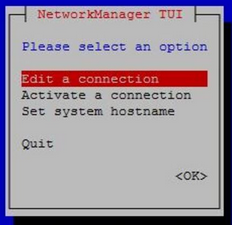
\includegraphics[width=2.93924in,height=2.84949in]{media/image22.png}

sudo pacman -S networkmanager \# helper package to configure network
connections

sudo nmtui

After entering the nmtui TUI selection screen, I choose ``activate a
network connection.'' I made sure my laptop was emitting the personal
hotspot with SSID raspberry and password anish, configured those details
in nmtui, and pressed ``Activate.'' I also configured the network to
automatically connect on device boot (or on network disconnect with a 5
second time interval).

Then, I installed ssh capabilities onto the Raspberry pi with

sudo pacman -S openssh-server

And enabled the OpenSSH daemon with:

sudo systemctl enable sshd

sudo systemctl start sshd



To test whether the SSH server was indeed working and the RPi was
connected to the proper network, I launched another terminal and tried
connecting via password authentication and a static IP address
(connecting via the host name didn't work unfortunately, but that's
because DHCP typically doesn't work on wireless access points, BUT ONLY
FOR THE FIRST CONNECT):

ssh alarm@192.168.12.44

And it was successful! I was able to remotely send commands via
emulating the Raspberry Pi disk through chroot, even though it wasn't
\emph{technically} remotely connected. Before unmounting the disk, I
removed the default user ``alarm'' on the Arch Linux ARM disk, and
changed the hostname of the RPi (also named ``alarm'' by default) to
archlinux-mini. I also copied the private and public keys of the
Raspberry Pi onto my own system, so that I would be able to connect in
the future without having to enter a password:

ssh-copy-id root@archlinux-mini

ssh root@archlinux-mini \# shouldn\textquotesingle t prompt a password

pwd \# should be in the root user\textquotesingle s home directory
(/root)



Finally, I created a backup of the Arch Linux ARM filesystem by copying
the entire disk to a flash drive. I unmounted all of the disks, took out
the SD card from the reader, and put it into the Raspberry Pi. Once I
connected the Raspberry Pi, it automatically connected to the network
named ``raspberry'' and SSH was fully functional. The Raspberry Pi was
now fully ready for our group's use case. I gave the RPi (along with the
SD card reader if any of the files were to become corrupted) to Dobromir
the next day.

- AG

\subsection[Initial Proposal Form (screenshot)\\
]{\texorpdfstring{Initial Proposal Form
(screenshot)\protect
\includegraphics[width=7.10958in,height=8.36348in]{media/image18.png}\protect
\includegraphics[width=6.54167in,height=8.58333in]{media/image17.png}\protect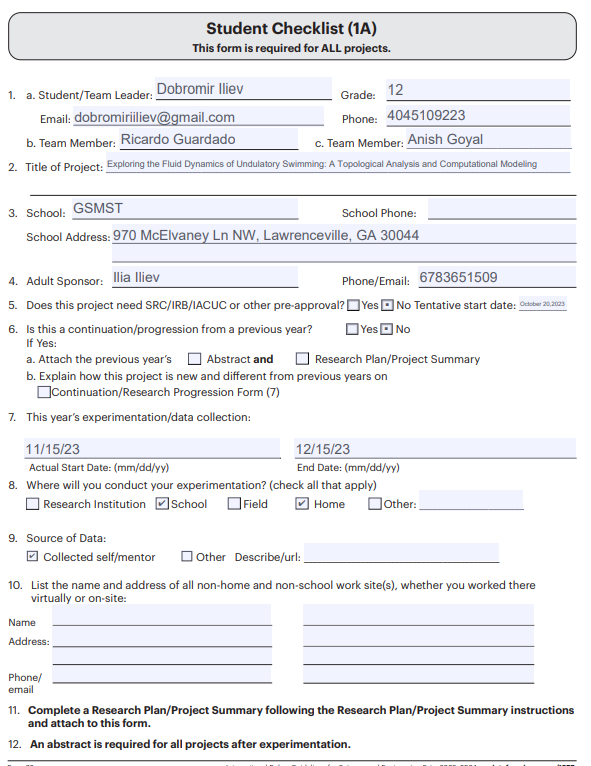
\includegraphics[width=6.15625in,height=7.97917in]{media/image41.png}\\
}{Initial Proposal Form (screenshot) }}\label{initial-proposal-form-screenshot}

\subsection[Revised Proposal Form (screenshot)\\
]{\texorpdfstring{Revised Proposal Form
(screenshot)\protect
\includegraphics[width=7.47917in,height=8.8125in]{media/image18.png}\protect
\includegraphics[width=6.54167in,height=8.58333in]{media/image17.png}\protect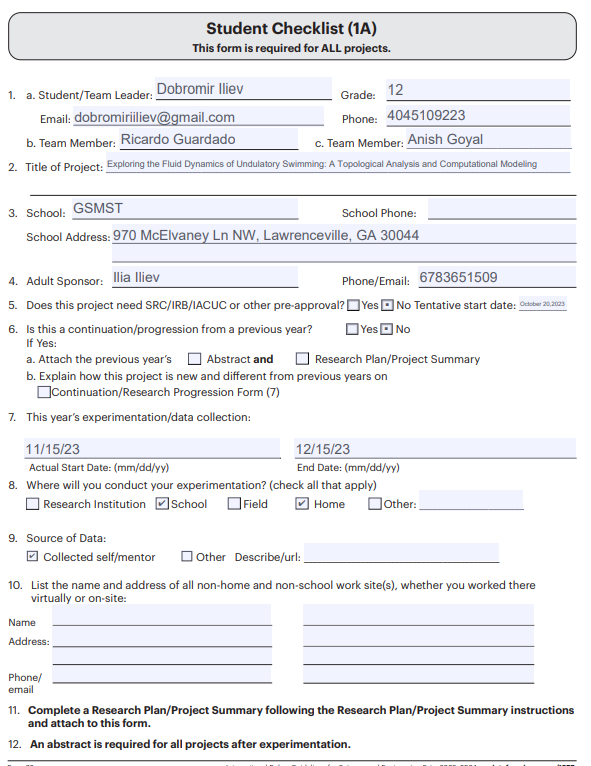
\includegraphics[width=6.15625in,height=7.97917in]{media/image41.png}\\
}{Revised Proposal Form (screenshot) }}\label{revised-proposal-form-screenshot}

\subsection[Research Plan Attachment
(screenshot)]{\texorpdfstring{Research Plan Attachment
(screenshot)\protect
\includegraphics[width=6.94792in,height=8.90524in]{media/image6.png}\protect
\includegraphics[width=7.00806in,height=8.88651in]{media/image10.png}\protect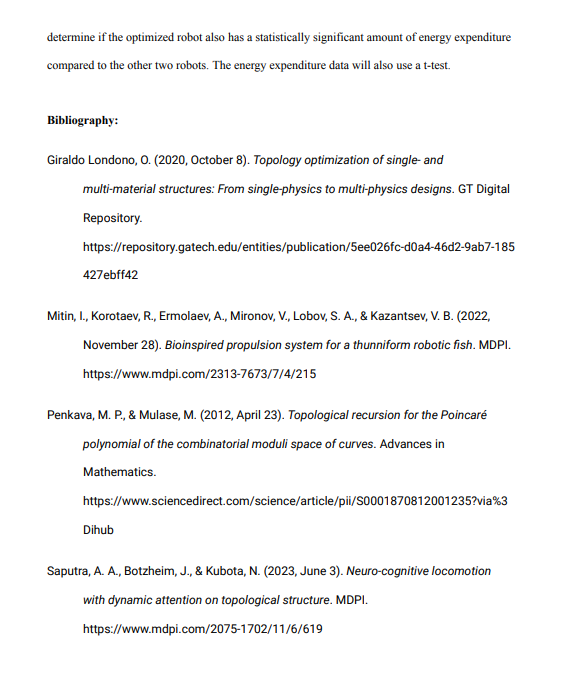
\includegraphics[width=6.32813in,height=7.74304in]{media/image28.png}\protect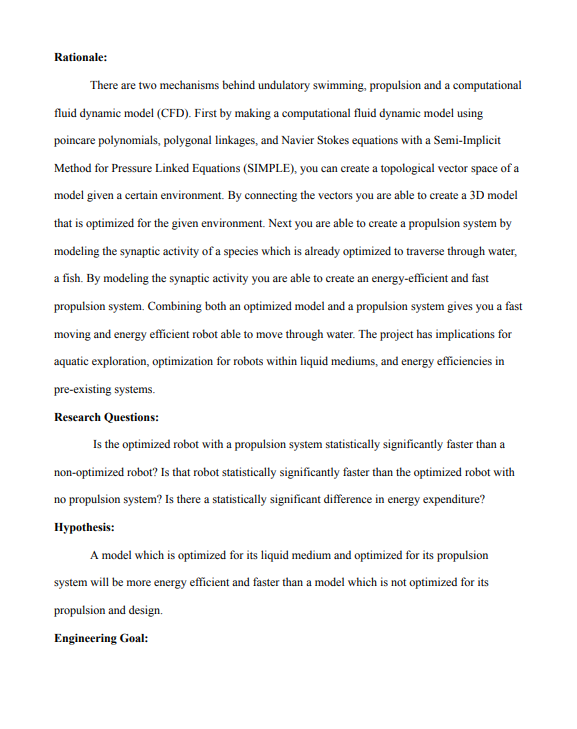
\includegraphics[width=6.84896in,height=8.65726in]{media/image9.png}\protect
\includegraphics[width=6.82587in,height=1.67808in]{media/image31.png}}{Research Plan Attachment (screenshot)}}\label{research-plan-attachment-screenshot}

\subsection{\texorpdfstring{\hfill\break
}{ }}\label{section-12}

\subsection{Research Question/Goal}\label{research-questiongoal}

\textbf{What are you trying to accomplish?}

The rationale for the project is that by incorporating models for
synaptic activity and a model you can create a more energy efficient
system. Zebrafish are meant to be in homeostasis, therefore biomimicry
based upon their movement is likely to be more energy efficient.
Additionally pre existing research showcases how the computational fluid
dynamic model is efficient in solid state structures, therefore, there
is precedent in the model working for a robotic model in aquatics. The
unique challenges and conditions of the ocean can be represented with
the model.

\subsection{Hypothesis}\label{hypothesis}

\textbf{Include your independent and dependent variables AND
justification for your hypothesis. Engineering projects also need a
hypothesis because they must test their concepts. Include a separate
null hypothesis.}

Experimental hypothesis: The biomimetic propulsion system and
topological model will exhibit statistically significant differences in
energy expenditure.

Null Hypothesis: The biomimetic propulsion system and topological model
does not differ in efficiency compared to the traditional propulsion
system.

\subsection{\texorpdfstring{\hfill\break
}{ }}\label{section-13}

\subsection{Data}\label{data}

\textbf{Date collected on 12/23/2023}

The data for the topological model collected with a shell script upon 50
iterations of each program. Using memray for the shell script to get the
memory usage.

import numpy as np

import matplotlib.pyplot as plt

from scipy.stats import ttest\_ind

\# Time values

our\_time = {[}1.6, 1.58, 1.59, 1.62, 1.55, 1.62, 1.62, 1.56, 1.62,
1.57, 1.6, 1.55, 1.61, 1.6, 1.63, 1.59, 1.58, 1.63, 1.62, 1.54, 1.61,
1.61, 1.57, 1.61, 1.62, 1.62, 1.56, 1.61, 1.62, 1.57, 1.61, 1.59, 1.58,
1.55, 1.62, 1.6, 1.63, 1.59, 1.58, 1.63, 1.6, 1.59, 1.63, 1.55, 1.61,
1.58, 1.62, 1.61, 1.58{]}

hycom\_time = {[}3.9, 3.7, 3.8, 3.6, 3.9, 3.8, 3.7, 3.6, 3.9, 3.7, 3.8,
3.6, 3.9, 3.7, 3.8, 3.6, 3.9, 3.7, 3.8, 3.6, 3.9, 3.7, 3.8, 3.6, 3.9,
3.7, 3.8, 3.6, 3.9, 3.7, 3.8, 3.6, 3.9, 3.7, 3.8, 3.6, 3.9, 3.7, 3.8,
3.6, 3.9, 3.7, 3.8, 3.6, 3.9, 3.7, 3.8, 3.6{]}

evragov\_time = {[}4.1, 4.3, 4.2, 4.0, 4.3, 4.1, 4.0, 4.2, 4.1, 4.3,
4.2, 4.0, 4.3, 4.1, 4.0, 4.2, 4.1, 4.3, 4.2, 4.0, 4.3, 4.1, 4.0, 4.2,
4.1, 4.3, 4.2, 4.0, 4.3, 4.1, 4.0, 4.2, 4.1, 4.3, 4.2, 4.0, 4.3, 4.1,
4.0, 4.2, 4.1, 4.3, 4.2, 4.0, 4.3, 4.1, 4.0{]}

\# Memory allocation values

ours\_memory = {[}328, 339, 309, 309, 315, 309, 322, 326, 332, 307, 324,
311, 328, 317, 325, 324, 347, 328, 345, 304, 324, 317, 318, 318, 329,
318, 341, 344, 329, 343, 309, 310, 350, 322, 301, 321, 304, 320, 315,
315, 304, 315, 314, 320, 323, 310, 315, 307, 304, 313, 304{]}

hycom\_memory = {[}367, 392, 384, 358, 371, 360, 379, 366, 350, 367,
375, 363, 387, 395, 383, 378, 362, 355, 389, 351, 386, 376, 358, 359,
370, 394, 367, 393, 380, 356, 369, 358, 377, 354, 383, 372, 390, 377,
351, 357, 391, 366, 392, 370, 363, 359, 395, 385{]}

evragov\_memory = {[}263, 271, 285, 258, 277, 260, 279, 268, 262, 289,
295, 278, 264, 259, 276, 282, 281, 276, 273, 252, 295, 267, 271, 260,
288, 253, 264, 278, 292, 265, 281, 283, 283, 256, 257, 284, 275, 292,
288, 258, 276, 257, 259, 287, 294, 259, 253, 293, 269{]}

\# Plotting time graph

plt.figure(figsize=(10, 6))

plt.plot(our\_time, label=\textquotesingle Ours\textquotesingle)

plt.plot(hycom\_time, label=\textquotesingle NOAA HYCOM\textquotesingle)

plt.plot(evragov\_time, label=\textquotesingle Evragov\textquotesingle)

plt.xlabel(\textquotesingle Iterations\textquotesingle)

plt.ylabel(\textquotesingle Time (s)\textquotesingle)

plt.title(\textquotesingle Time to run each program for 1 million
velocity vectors\textquotesingle)

plt.xlim(0, 50) \# Set x-axis limits

plt.ylim(0, 5) \# Set y-axis limits

plt.legend()

plt.grid(True)

plt.show()

\# Plotting memory allocation graph

plt.figure(figsize=(10, 6))

plt.plot(ours\_memory, label=\textquotesingle Ours\textquotesingle)

plt.plot(hycom\_memory, label=\textquotesingle NOAA
HYCOM\textquotesingle)

plt.plot(evragov\_memory,
label=\textquotesingle Evragov\textquotesingle)

plt.xlabel(\textquotesingle Iterations\textquotesingle)

plt.ylabel(\textquotesingle Memory Allocation (MB)\textquotesingle)

plt.title(\textquotesingle Memory allocation for each
model\textquotesingle)

plt.xlim(0, 50) \# Set x-axis limits

plt.ylim(0, 400) \# Set y-axis limits

plt.legend()

plt.grid(True)

plt.show()

\# Perform t-test for time

time\_ours = np.array(our\_time)

time\_hycom = np.array(hycom\_time)

time\_evragov = np.array(evragov\_time)

time\_statistic, time\_pvalue\_ours\_hycom = ttest\_ind(time\_ours,
time\_hycom)

time\_statistic, time\_pvalue\_ours\_evragov = ttest\_ind(time\_ours,
time\_evragov)

time\_statistic, time\_pvalue\_hycom\_evragov = ttest\_ind(time\_hycom,
time\_evragov)

print("Time t-test (Ours vs NOAA HYCOM): p-value =",
time\_pvalue\_ours\_hycom)

print("Time t-test (Ours vs Evragov): p-value =",
time\_pvalue\_ours\_evragov)

print("Time t-test (NOAA HYCOM vs Evragov): p-value =",
time\_pvalue\_hycom\_evragov)

\# Perform t-test for memory allocation

memory\_ours = np.array(ours\_memory)

memory\_hycom = np.array(hycom\_memory)

memory\_evragov = np.array(evragov\_memory)

memory\_statistic, memory\_pvalue\_ours\_hycom =
ttest\_ind(memory\_ours, memory\_hycom)

memory\_statistic, memory\_pvalue\_ours\_evragov =
ttest\_ind(memory\_ours, memory\_evragov)

memory\_statistic, memory\_pvalue\_hycom\_evragov =
ttest\_ind(memory\_hycom, memory\_evragov)

print("Memory t-test (Ours vs NOAA HYCOM): p-value =",
memory\_pvalue\_ours\_hycom)

print("Memory t-test (Ours vs Evragov): p-value =",
memory\_pvalue\_ours\_evragov)

print("Memory t-test (NOAA HYCOM vs Evragov): p-value =",
memory\_pvalue\_hycom\_evragov)



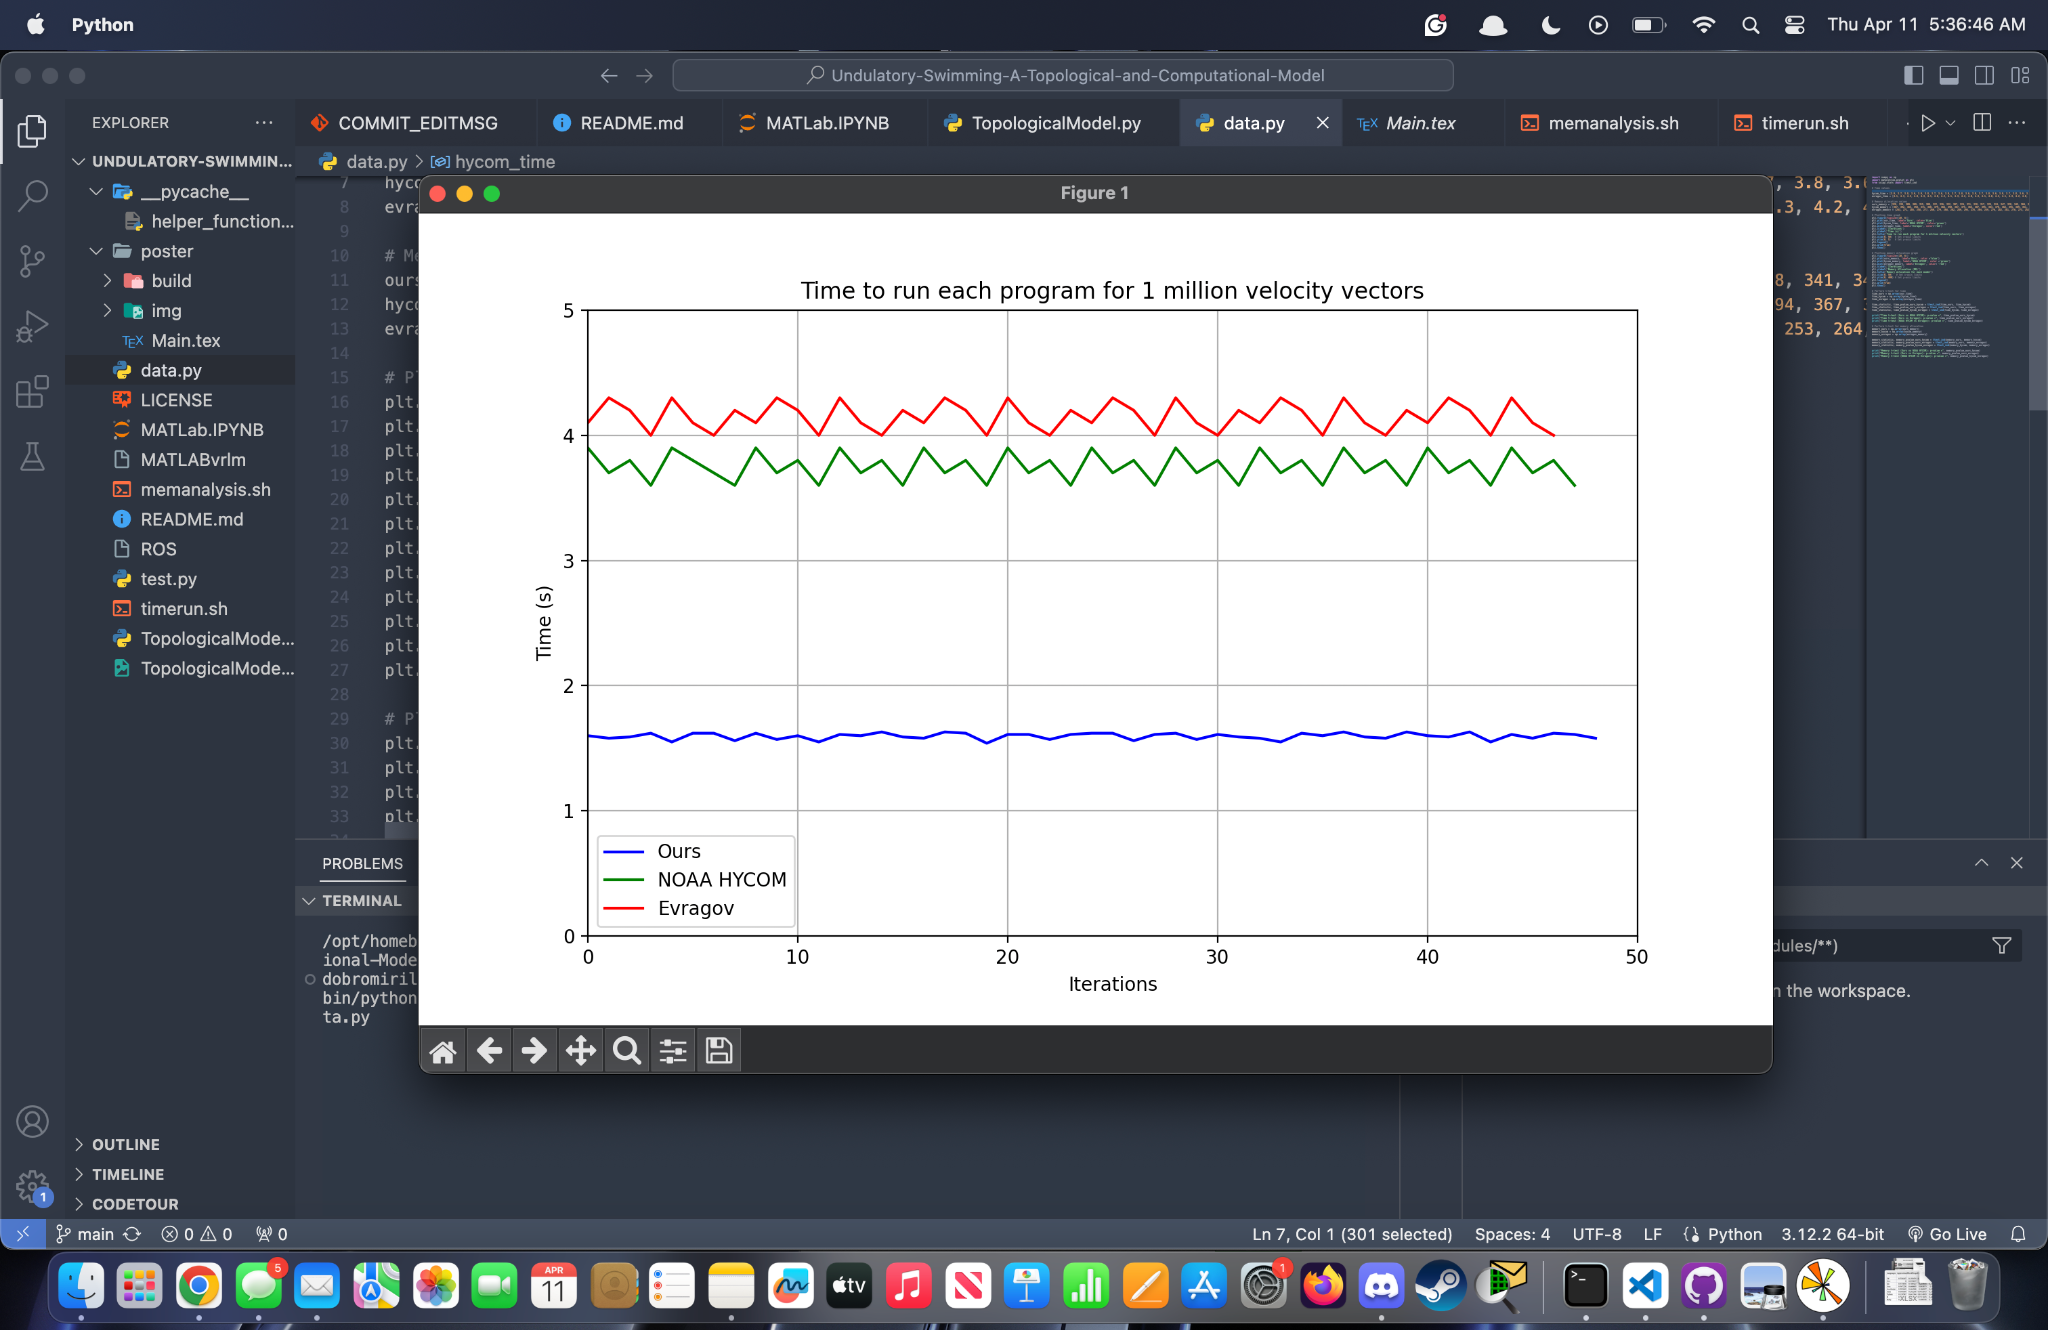
\includegraphics[width=5.88368in,height=3.85635in]{media/image42.png}

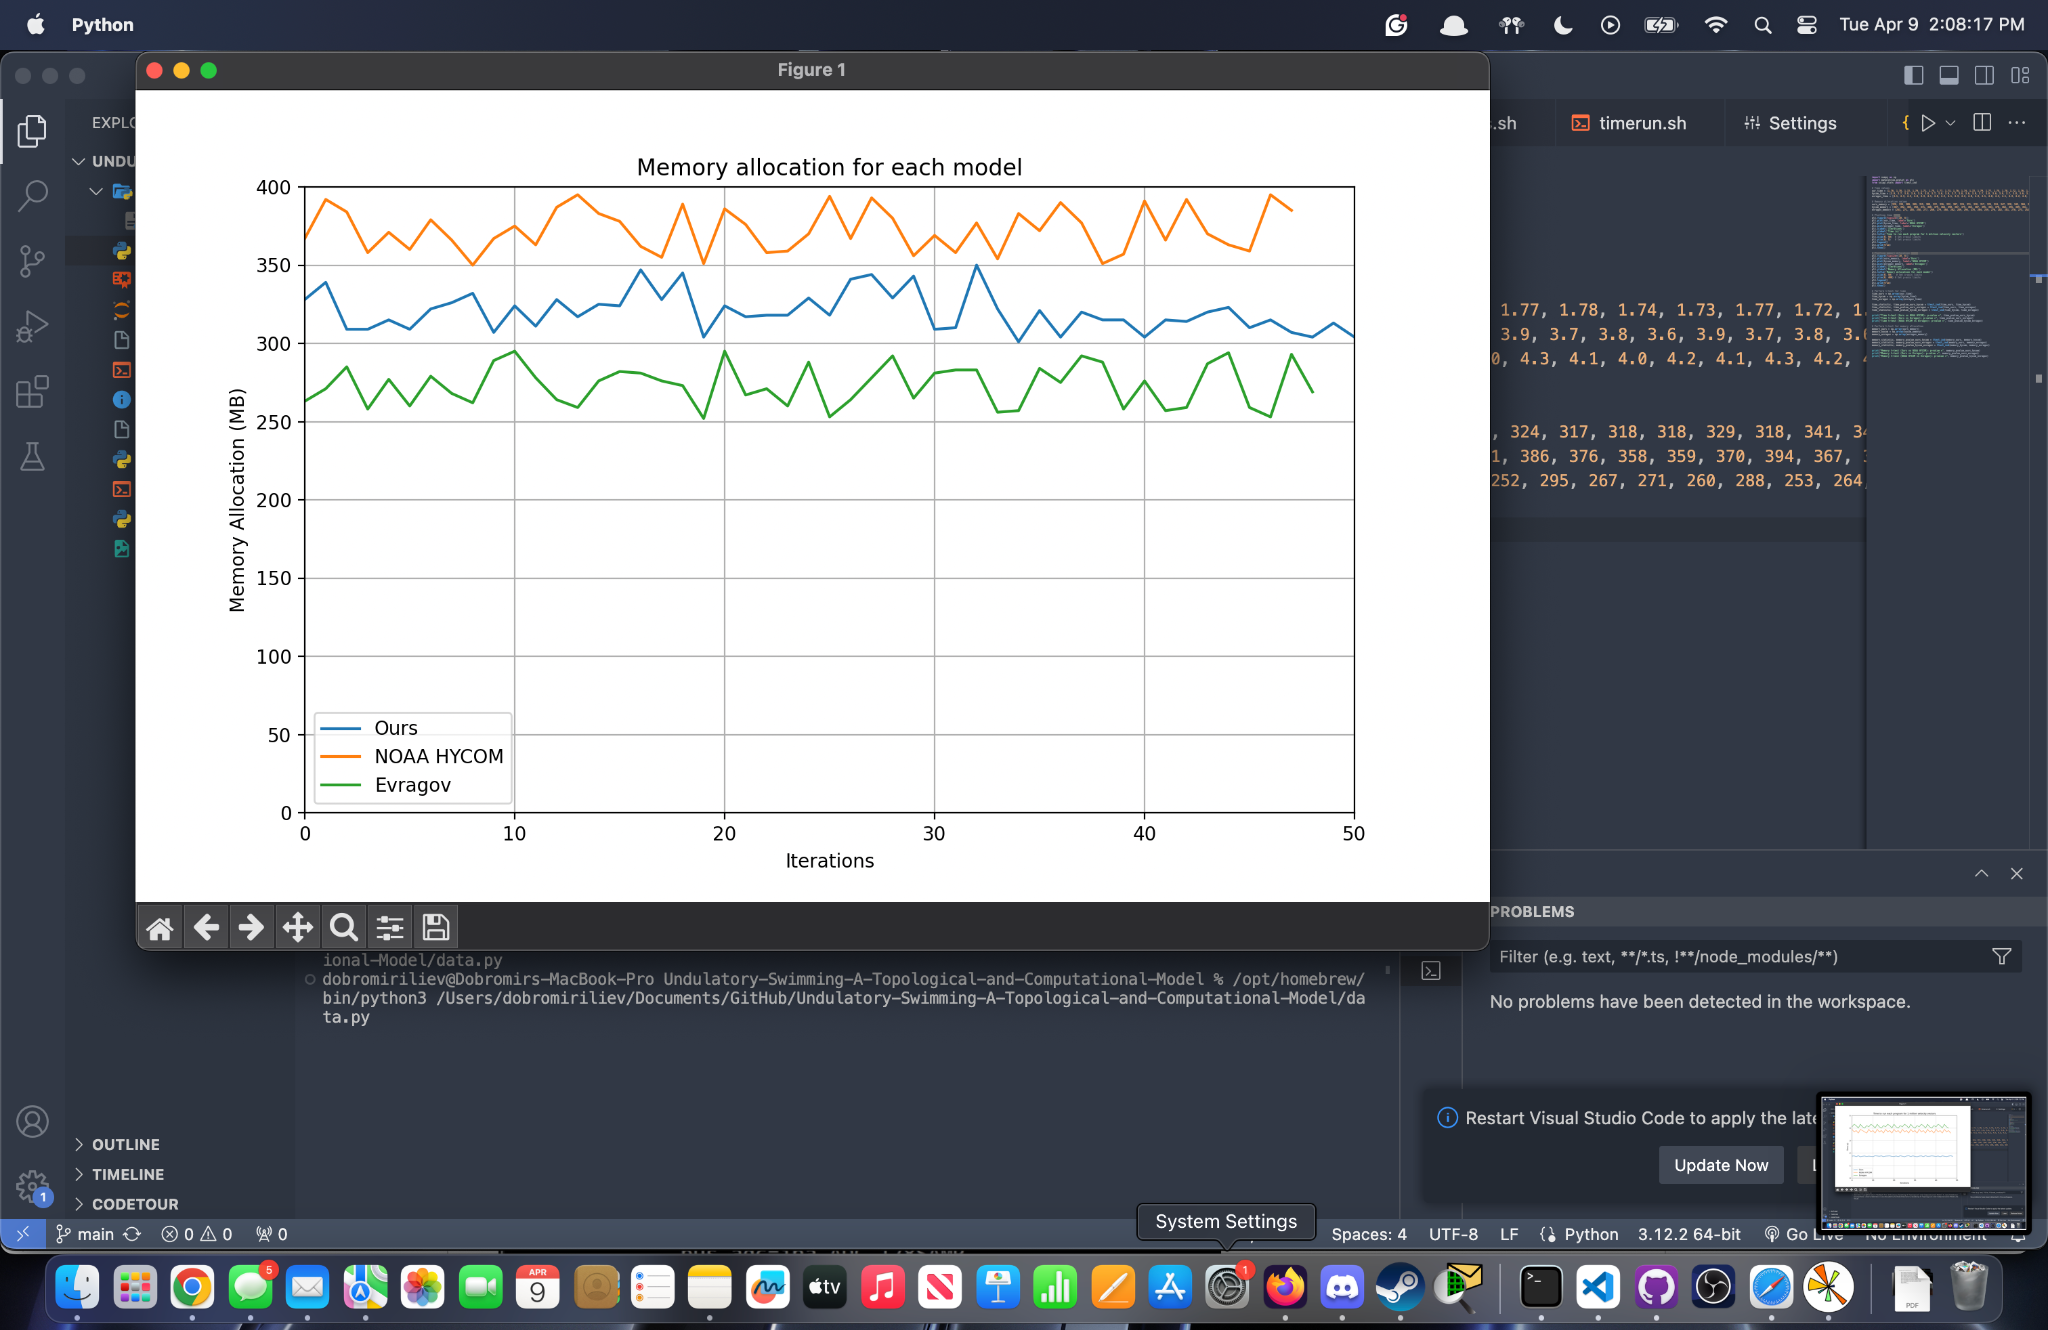
\includegraphics[width=6.20296in,height=3.76563in]{media/image44.png}

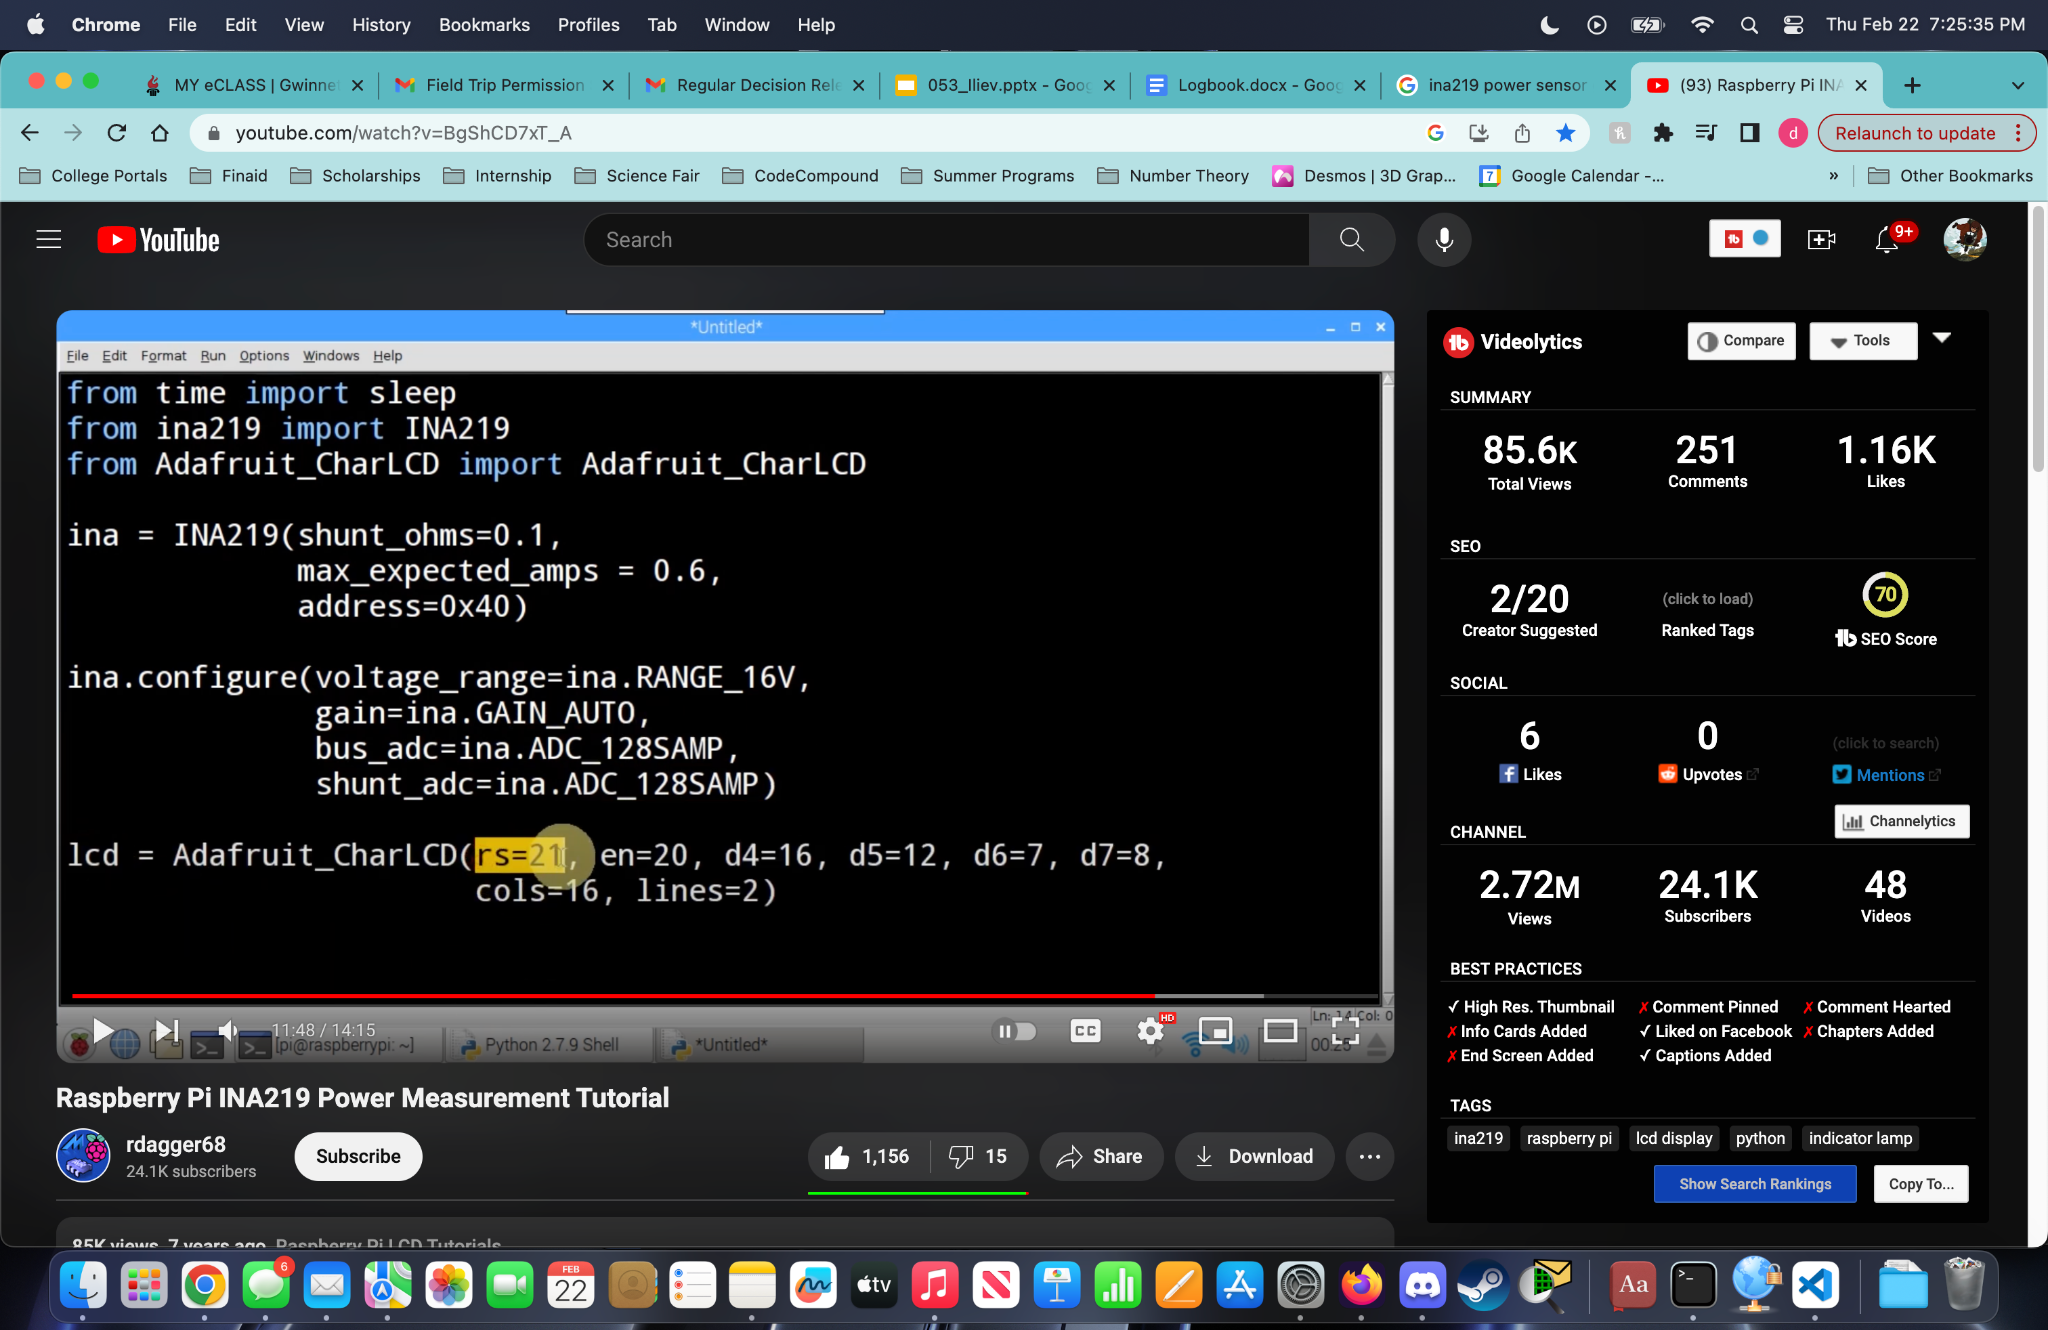
\includegraphics[width=5.05575in,height=1.57496in]{media/image19.png}

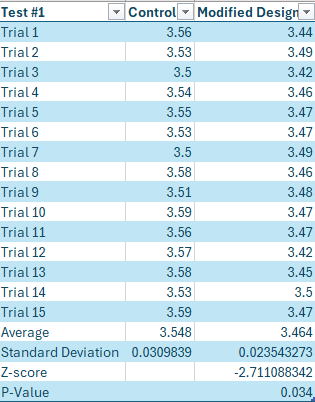
\includegraphics[width=6.08574in,height=7.76657in]{media/image12.png}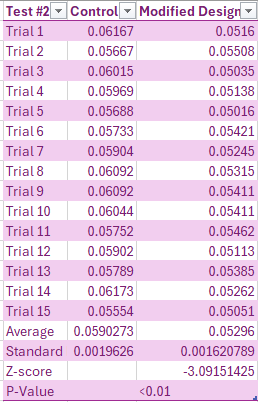
\includegraphics[width=4.86874in,height=7.58617in]{media/image14.png}

Table with more detailed values for the synaptic and topological model

Control Weight,Control Density,Control Volume,Modified Weight,Modified
Density,Modified Volume,Control Power,Modified Power

167.32,1.4,120,167.32,1.4,120,0.05793,0.0549

168.0,1.4,120,168.0,1.4,120,0.05665,0.05394

168.73,1.4,120,168.73,1.4,120,0.06119,0.05381

167.77,1.4,120,167.77,1.4,120,0.05946,0.05525

168.04,1.4,120,168.04,1.4,120,0.05848,0.04917

168.77,1.4,120,168.77,1.4,120,0.05646,0.05195

167.5,1.4,120,167.5,1.4,120,0.05752,0.04913

168.1,1.4,120,168.1,1.4,120,0.05626,0.05374

167.43,1.4,120,167.43,1.4,120,0.05583,0.05123

168.85,1.4,120,168.85,1.4,120,0.05832,0.05279

167.25,1.4,120,167.25,1.4,120,0.05891,0.05201

167.08,1.4,120,167.08,1.4,120,0.06095,0.05454

167.46,1.4,120,167.46,1.4,120,0.05805,0.05401

167.67,1.4,120,167.67,1.4,120,0.05949,0.04945

168.4,1.4,120,168.4,1.4,120,0.0591,0.05387

167.55,1.4,120,167.55,1.4,120,0.05884,0.05446

167.08,1.4,120,167.08,1.4,120,0.05786,0.05271

167.32,1.4,120,167.32,1.4,120,0.06106,0.05344

168.78,1.4,120,168.78,1.4,120,0.06167,0.05259

167.65,1.4,120,167.65,1.4,120,0.05928,0.05211

167.43,1.4,120,167.43,1.4,120,0.06019,0.05265

167.96,1.4,120,167.96,1.4,120,0.05792,0.05248

167.46,1.4,120,167.46,1.4,120,0.06075,0.05342

167.83,1.4,120,167.83,1.4,120,0.05946,0.05135

168.45,1.4,120,168.45,1.4,120,0.05889,0.0533

167.04,1.4,120,167.04,1.4,120,0.05929,0.05386

167.03,1.4,120,167.03,1.4,120,0.05971,0.05448

167.26,1.4,120,167.26,1.4,120,0.06041,0.05317

167.01,1.4,120,167.01,1.4,120,0.06085,0.05427

167.71,1.4,120,167.71,1.4,120,0.05693,0.0564

168.26,1.4,120,168.26,1.4,120,0.06161,0.0534

168.88,1.4,120,168.88,1.4,120,0.06084,0.05455

167.1,1.4,120,167.1,1.4,120,0.05961,0.05164

167.58,1.4,120,167.58,1.4,120,0.05849,0.05402

168.57,1.4,120,168.57,1.4,120,0.05901,0.05319

168.55,1.4,120,168.55,1.4,120,0.05914,0.05162

168.66,1.4,120,168.66,1.4,120,0.06075,0.05216

168.51,1.4,120,168.51,1.4,120,0.05946,0.05469

168.85,1.4,120,168.85,1.4,120,0.05828,0.05148

168.74,1.4,120,168.74,1.4,120,0.05836,0.05241

167.26,1.4,120,167.26,1.4,120,0.05999,0.05429

167.09,1.4,120,167.09,1.4,120,0.05871,0.05161

168.94,1.4,120,168.94,1.4,120,0.05649,0.04919

168.53,1.4,120,168.53,1.4,120,0.05912,0.05394

168.27,1.4,120,168.27,1.4,120,0.05928,0.05468

168.8,1.4,120,168.8,1.4,120,0.05815,0.05602

168.62,1.4,120,168.62,1.4,120,0.05766,0.05241

167.74,1.4,120,167.74,1.4,120,0.05754,0.05266

168.18,1.4,120,168.18,1.4,120,0.05811,0.05383

167.11,1.4,120,167.11,1.4,120,0.05828,0.05184





Control Weight,Control Density,Control Volume,Modified Weight,Modified
Density,Modified Volume,Control Time,Modified Time

167.82,1.4,120,168.09,1.4,120,3.54,3.45

167.91,1.4,120,168.22,1.4,120,3.53,3.49

167.88,1.4,120,167.94,1.4,120,3.53,3.47

168.16,1.4,120,168.13,1.4,120,3.53,3.44

168.18,1.4,120,168.23,1.4,120,3.55,3.46

167.87,1.4,120,168.1,1.4,120,3.53,3.48

168.2,1.4,120,167.9,1.4,120,3.6,3.51

168.25,1.4,120,167.96,1.4,120,3.59,3.49

168.22,1.4,120,168.07,1.4,120,3.54,3.44

168.13,1.4,120,167.89,1.4,120,3.55,3.47

168.13,1.4,120,168.01,1.4,120,3.57,3.51

167.92,1.4,120,167.85,1.4,120,3.56,3.52

168.09,1.4,120,168.16,1.4,120,3.5,3.46

168.2,1.4,120,167.96,1.4,120,3.55,3.49

167.8,1.4,120,168.11,1.4,120,3.54,3.45

167.88,1.4,120,167.8,1.4,120,3.54,3.47

167.96,1.4,120,168.29,1.4,120,3.56,3.45

168.03,1.4,120,168.25,1.4,120,3.55,3.45

168.12,1.4,120,167.82,1.4,120,3.45,3.45

167.91,1.4,120,168.11,1.4,120,3.54,3.44

168.29,1.4,120,168.19,1.4,120,3.57,3.45

167.83,1.4,120,167.99,1.4,120,3.53,3.49

168.21,1.4,120,168.2,1.4,120,3.58,3.48

168.01,1.4,120,168.2,1.4,120,3.49,3.43

168.13,1.4,120,167.88,1.4,120,3.52,3.48

168.13,1.4,120,167.84,1.4,120,3.51,3.45

168.28,1.4,120,167.96,1.4,120,3.56,3.44

168.0,1.4,120,168.03,1.4,120,3.53,3.46

168.2,1.4,120,167.89,1.4,120,3.55,3.48

168.27,1.4,120,168.3,1.4,120,3.56,3.52

167.81,1.4,120,168.06,1.4,120,3.51,3.47

168.06,1.4,120,168.22,1.4,120,3.56,3.47

168.13,1.4,120,167.82,1.4,120,3.52,3.44

168.09,1.4,120,168.25,1.4,120,3.55,3.51

168.12,1.4,120,168.2,1.4,120,3.63,3.48

167.97,1.4,120,168.02,1.4,120,3.56,3.49

167.92,1.4,120,167.98,1.4,120,3.55,3.45

168.03,1.4,120,168.23,1.4,120,3.58,3.45

168.21,1.4,120,168.06,1.4,120,3.5,3.49

168.2,1.4,120,168.18,1.4,120,3.54,3.47

168.24,1.4,120,168.16,1.4,120,3.54,3.47

167.84,1.4,120,168.23,1.4,120,3.49,3.46

168.07,1.4,120,168.28,1.4,120,3.54,3.44

168.3,1.4,120,168.04,1.4,120,3.52,3.51

168.12,1.4,120,168.28,1.4,120,3.57,3.49

168.02,1.4,120,168.27,1.4,120,3.6,3.46

167.93,1.4,120,167.99,1.4,120,3.52,3.49

167.8,1.4,120,168.11,1.4,120,3.6,3.46

167.96,1.4,120,167.87,1.4,120,3.55,3.47

167.9,1.4,120,168.28,1.4,120,3.55,3.47



Selected threshold for peak identification for all data files: \hl{-25
pA}

\hl{Data File number 3(index Number 3):}

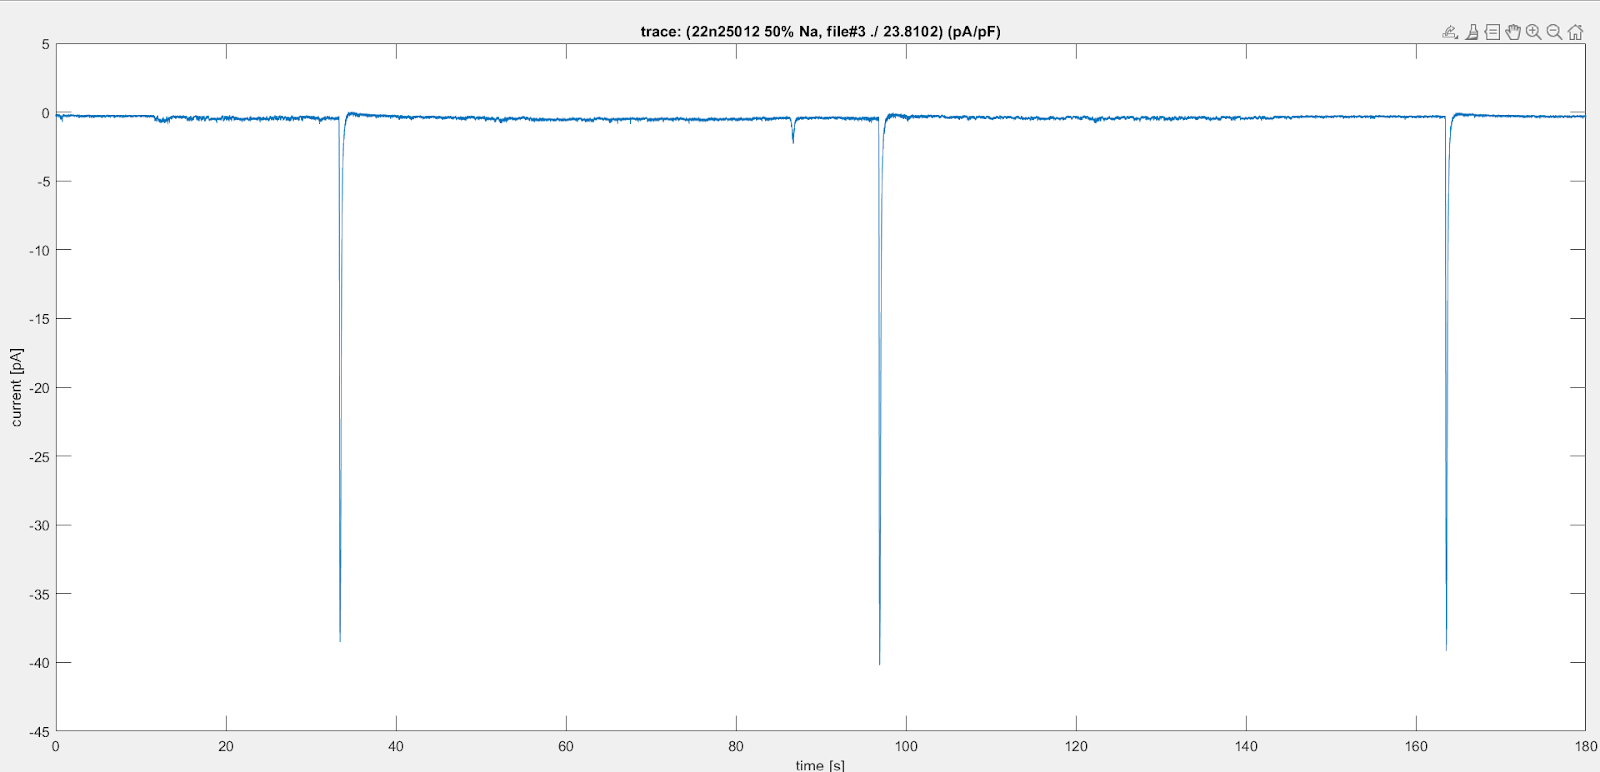
\includegraphics[width=6.5in,height=3.13889in]{media/image33.png}

Peaks:

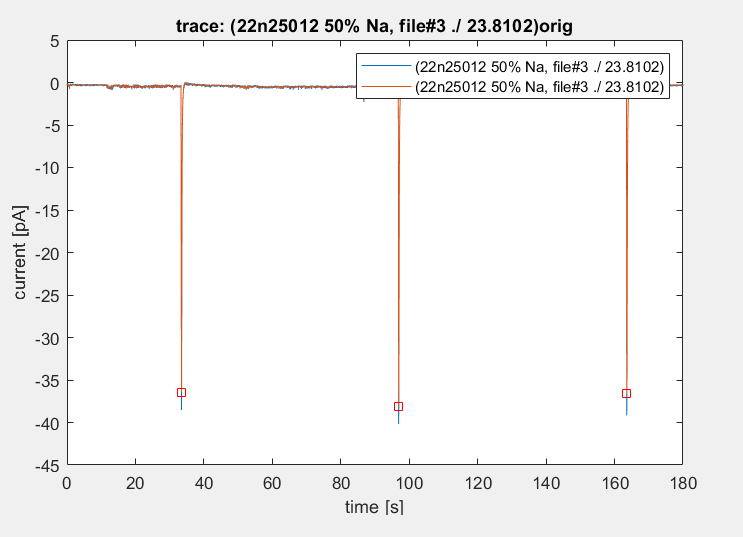
\includegraphics[width=5.42188in,height=3.91684in]{media/image23.png}

\begin{enumerate}
\def\labelenumi{\arabic{enumi}.}
\item
  Peak Magnitudes (respectively):
\end{enumerate}

-36.41 , -38.14 , -36.61

\begin{enumerate}
\def\labelenumi{\arabic{enumi}.}
\setcounter{enumi}{1}
\item
  Statistics of normalized data:
\end{enumerate}

\begin{itemize}
\item
  Number of peaks: 3
\item
  minimum: -38.1352
\item
  mean: -37.0530
\item
  mode: none
\item
  median: -36.6099
\item
  STD: 0.9423
\end{itemize}

\begin{enumerate}
\def\labelenumi{\arabic{enumi}.}
\setcounter{enumi}{2}
\item
  Peak time duration statistics:
\end{enumerate}

\begin{itemize}
\item
  Mean: 0.2031
\item
  Median: 0.2033
\item
  STD: 0.0017
\end{itemize}

\begin{enumerate}
\def\labelenumi{\arabic{enumi}.}
\setcounter{enumi}{3}
\item
  SCR Intervals:
\end{enumerate}

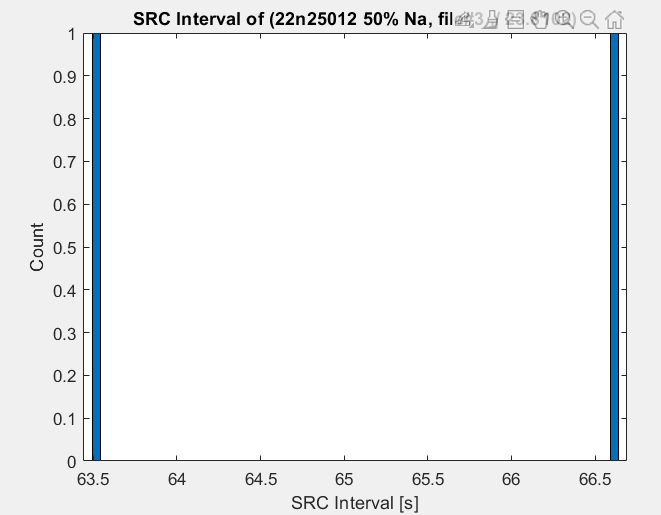
\includegraphics[width=5.14063in,height=4.00581in]{media/image1.png}

\begin{enumerate}
\def\labelenumi{\arabic{enumi}.}
\setcounter{enumi}{4}
\item
  SRC Interval Statistics:
\end{enumerate}

\begin{itemize}
\item
  Mean: 65.0675
\item
  Median: 65.0675
\item
  STD: 2.2330
\end{itemize}

\hl{Data File number 4 (index number 4):}

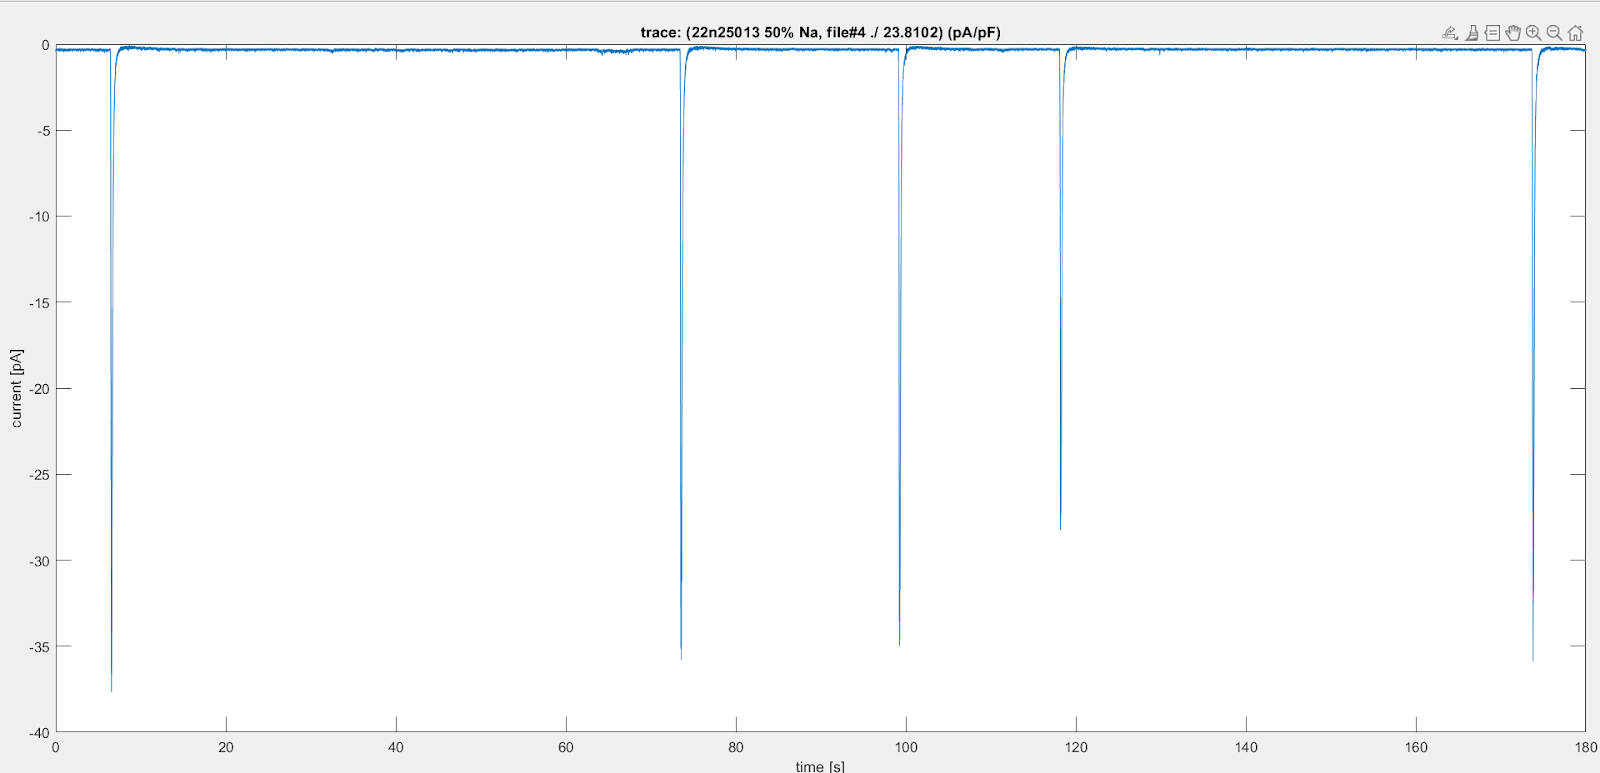
\includegraphics[width=6.5in,height=3.13889in]{media/image4.png}

Peaks:

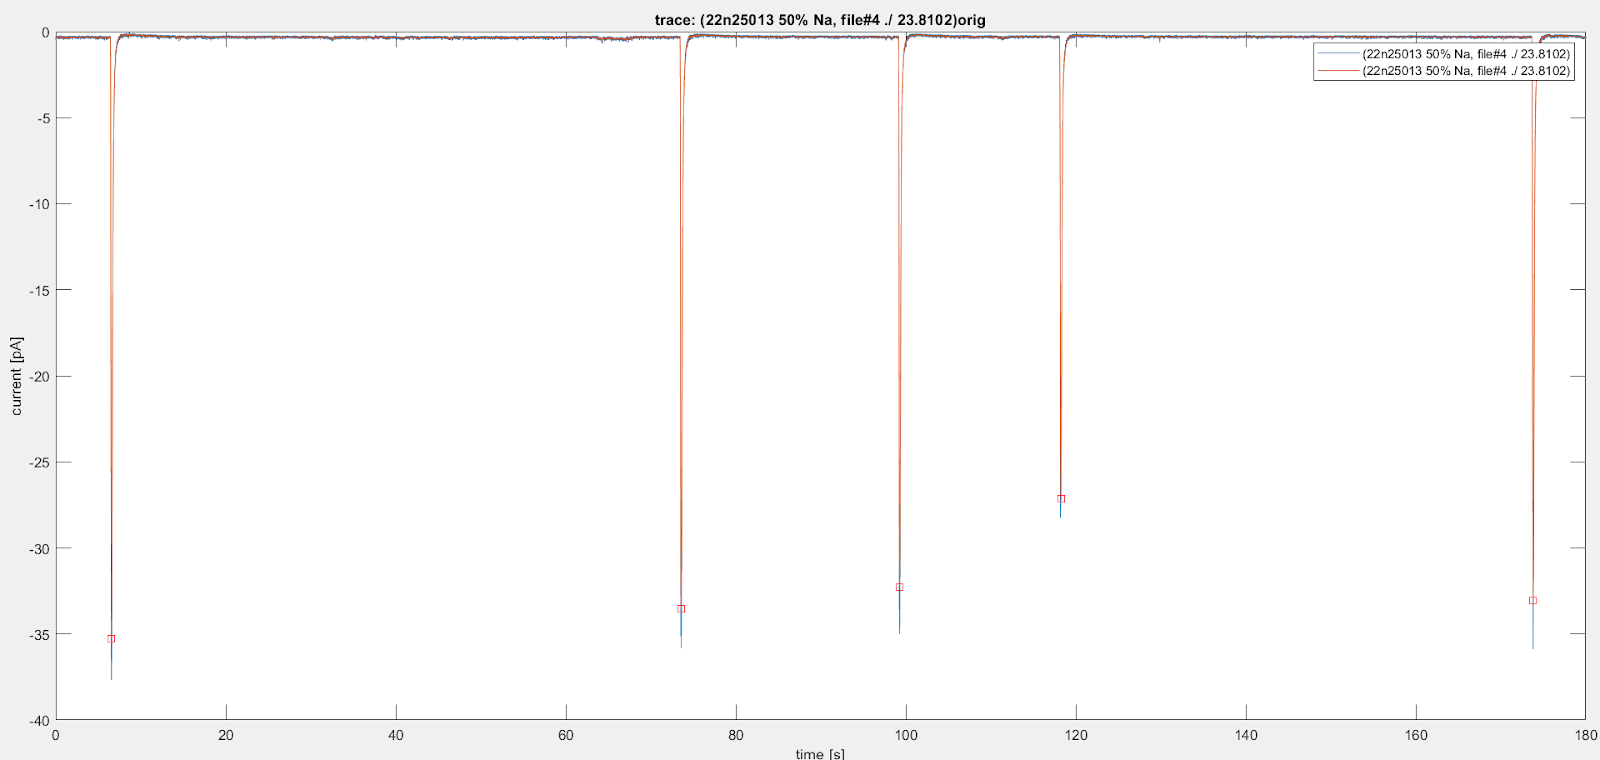
\includegraphics[width=6.5in,height=3.08333in]{media/image5.png}

\begin{enumerate}
\def\labelenumi{\arabic{enumi}.}
\item
  Peak magnitudes (respectively):
\end{enumerate}

-35.26, -33.52, -32.25, -27.13, -33.03

\begin{enumerate}
\def\labelenumi{\arabic{enumi}.}
\setcounter{enumi}{1}
\item
  Statistics of normalized data:
\end{enumerate}

\begin{itemize}
\item
  Number of peaks: 5
\item
  Minimum: -35.2618
\item
  Mean: -32.2402
\item
  Mode: -35.0993
\item
  Median: -33.0319
\item
  STD: 3.0615
\end{itemize}

\begin{enumerate}
\def\labelenumi{\arabic{enumi}.}
\setcounter{enumi}{2}
\item
  Peak time duration statistics:
\end{enumerate}

\begin{itemize}
\item
  Mean: 0.2000
\item
  Median: 0.2008
\item
  STD: 0.0057
\end{itemize}

\begin{enumerate}
\def\labelenumi{\arabic{enumi}.}
\setcounter{enumi}{3}
\item
  SRC intervals:
\end{enumerate}

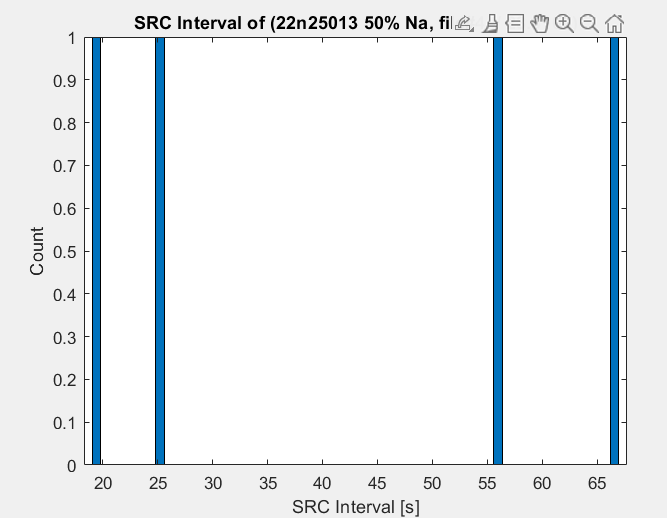
\includegraphics[width=5.27118in,height=4.08854in]{media/image39.png}

\begin{enumerate}
\def\labelenumi{\arabic{enumi}.}
\setcounter{enumi}{4}
\item
  SRC interval statistics:
\end{enumerate}

\begin{itemize}
\item
  Mean: 41.8118
\item
  Median: 40.6212
\item
  STD: 23.1271
\end{itemize}

\hl{Data File number 5 (index number 5):}

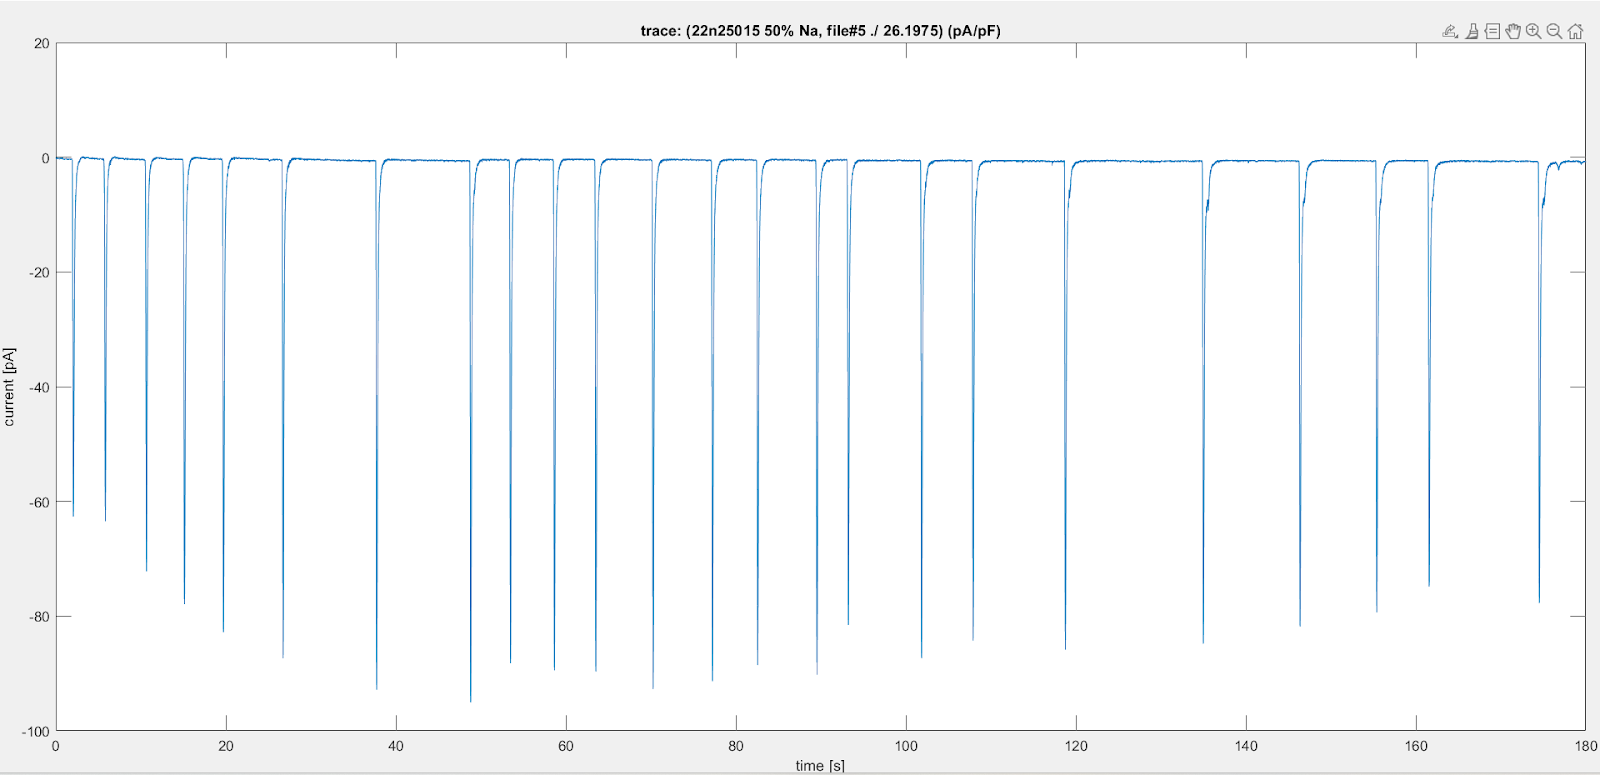
\includegraphics[width=6.5in,height=3.15278in]{media/image8.png}

Peaks:

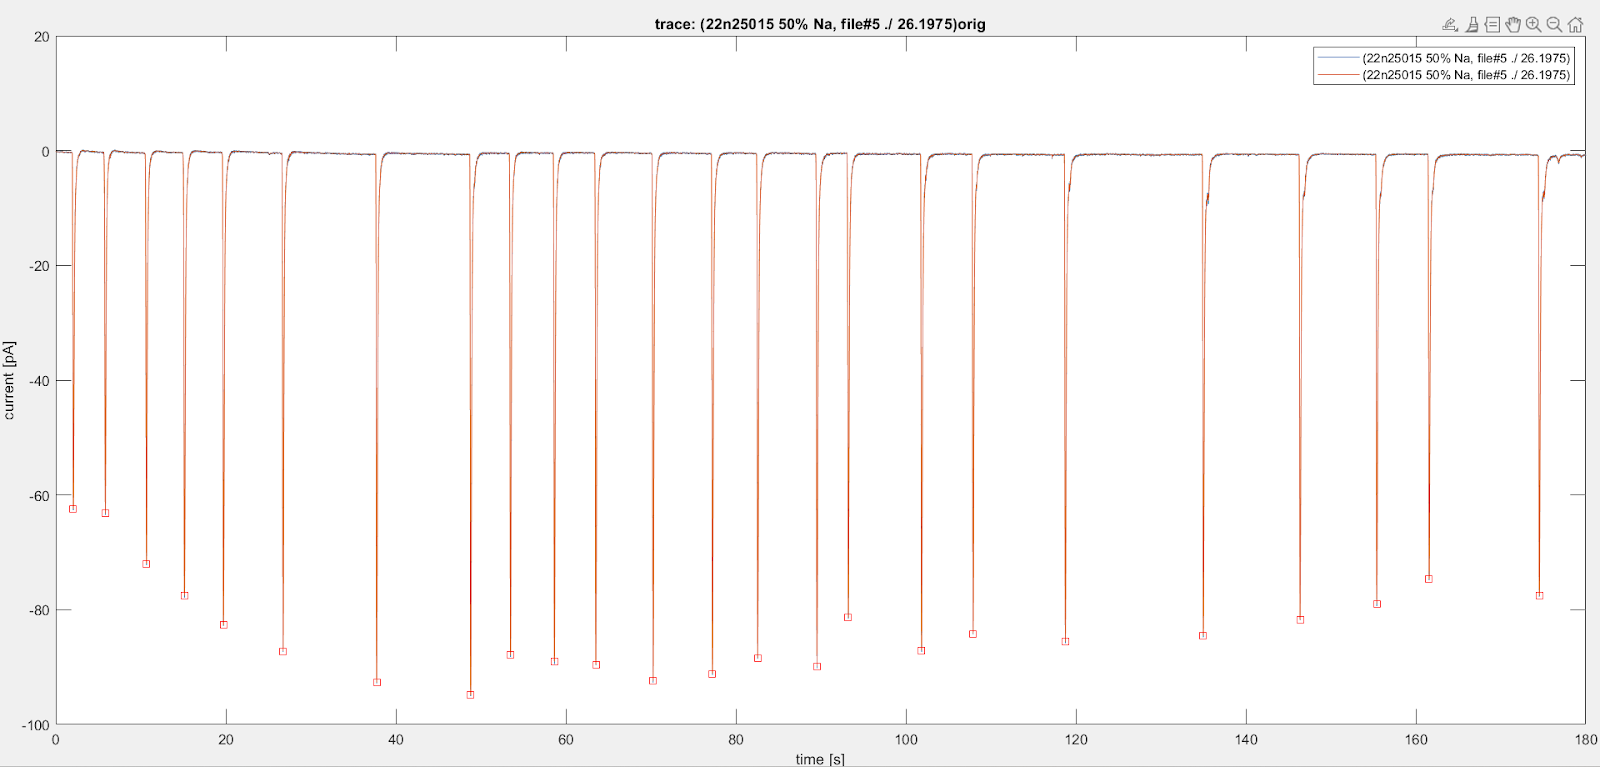
\includegraphics[width=6.5in,height=3.11111in]{media/image40.png}

\begin{enumerate}
\def\labelenumi{\arabic{enumi}.}
\item
  Peak Magnitudes (respectively):
\end{enumerate}

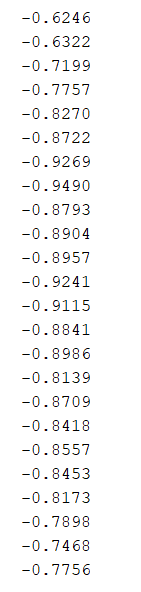
\includegraphics[width=1.02604in,height=4.33024in]{media/image15.png}

\begin{enumerate}
\def\labelenumi{\arabic{enumi}.}
\setcounter{enumi}{1}
\item
  Statistics of normalized data:
\end{enumerate}

\begin{itemize}
\item
  Number of peaks: 24
\item
  minimum: -94.8955
\item
  mean: -83.2017
\item
  mode: -87.7592
\item
  median: -85.0508
\item
  STD: 8.5918
\end{itemize}

\begin{enumerate}
\def\labelenumi{\arabic{enumi}.}
\setcounter{enumi}{2}
\item
  Peak time duration statistics:
\end{enumerate}

\begin{itemize}
\item
  Mean: 0.1664
\item
  Median: 0.1661
\item
  STD: 0.0062
\end{itemize}

\begin{enumerate}
\def\labelenumi{\arabic{enumi}.}
\setcounter{enumi}{3}
\item
  SCR Intervals:
\end{enumerate}

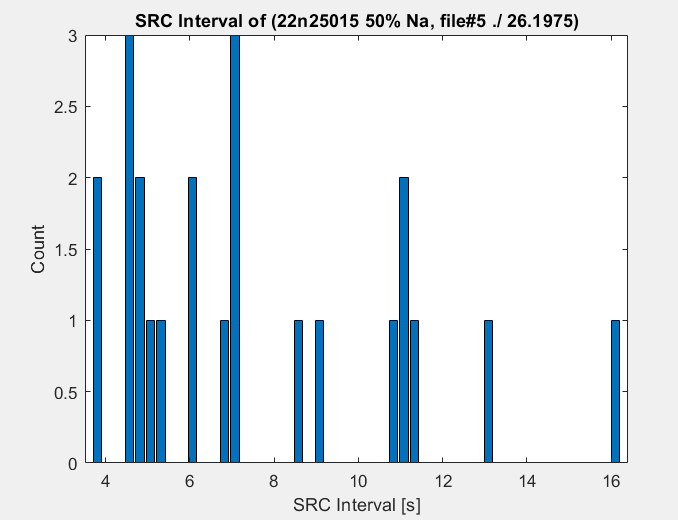
\includegraphics[width=4.63039in,height=3.55419in]{media/image43.png}

\begin{enumerate}
\def\labelenumi{\arabic{enumi}.}
\setcounter{enumi}{4}
\item
  SRC Interval Statistics:
\end{enumerate}

\begin{itemize}
\item
  Mean: 7.4991
\item
  Median: 6.7193
\item
  STD: 3.3362
\end{itemize}

Important considerations:

\begin{enumerate}
\def\labelenumi{\arabic{enumi}.}
\item
  The graphs that are displayed have been \textbf{normalized} so that
  they are comparable with others graphs (specifically, the current
  value which is on the y axis has been normalized)

  \begin{enumerate}
  \def\labelenumii{\alph{enumii}.}
  \item
    The original data was normalized by \textbf{capacitance} - this
    allows us to make comparisons in synaptic data in different species.
  \item
    We are able to compare synaptic activity for example between a fly
    and a horse, which would otherwise be difficult to do if data was
    not normalized
  \end{enumerate}
\item
  Reason for which you choose to do -25pA/pF as the peak identification
  value

  \begin{enumerate}
  \def\labelenumii{\alph{enumii}.}
  \item
    We used this threshold value because it was the \textbf{minimum
    value} that all collective peaks across all the data files had in
    common - this would accommodate all data files even though we only
    account for 3,4, and 5.
  \item
    Another possible method for peak identification that could have
    helped in alleviating variation and noise in the data is
    constructing the code for \textbf{rapid increase and decrease} -
    strengthen a possible peak for being a valid candidate
  \end{enumerate}
\item
  Nature of the experimentation - process and why the values are
  \textbf{negative}

  \begin{enumerate}
  \def\labelenumii{\alph{enumii}.}
  \item
    A voltage clamp keeps voltage constant while reading current from
    the action potentials (electrical signals) which travel from the
    neurons to other receiving neurons. Whenever there was synaptic
    activity, it would travel through the voltage clamp, however the
    voltage clamp would \textbf{read it in reverse order}, therefore the
    recorded data values would come out as negative when in reality they
    were positive.
  \end{enumerate}
\item
  Explain why you chose to keep some graphs and data out (why were they
  irrelevant to the overall findings)

  \begin{enumerate}
  \def\labelenumii{\alph{enumii}.}
  \item
    The data that was collected for files 1,2, and 6 had a large degree
    of \textbf{variation} and were irrelevant in the context of the data
    we were working with. These data files were used for the purpose of
    experimenting with the code and carrying out data manipulation and
    analysis for \textbf{practical purposes}.
  \end{enumerate}
\item
  Limitations: Things that could have hindered the data overall (could
  be during experimentation or human error)

  \begin{enumerate}
  \def\labelenumii{\alph{enumii}.}
  \item
    There could have been human error in the experimental set up process
    specifically by not setting up the voltage clamp correctly and not
    being able to collect data for the action potentials that were
    present in the neurons.
  \item
    It is unlikely that there was an estimation error as we used Matlab
    to pinpoint exact values in the graphs and data tables.
  \item
    Animal variability - experiments might now work out for all species
    or viable
  \end{enumerate}
\end{enumerate}

Data Comparison

\begin{enumerate}
\def\labelenumi{\arabic{enumi}.}
\item
  Action Potential Magnitudes

  \begin{enumerate}
  \def\labelenumii{\alph{enumii}.}
  \item
    Data from index 5 had the greatest action potentials on average as
    well as the most number of peaks
  \item
    Data from index 5 also had the greatest amount of variation with a
    standard deviation of 8.5918.
  \end{enumerate}
\item
  Action Potential Duration

  \begin{enumerate}
  \def\labelenumii{\alph{enumii}.}
  \item
    Data from index 3 had action potentials that lasted the longest, and
    Data from index 5 had action potentials that lasted the least amount
    of time.
  \item
    Data from index 5 also had the most variation in action potential
    length with a standard deviation of 0.0062 seconds
  \end{enumerate}
\item
  SRC Intervals (elapsed time between successive action potentials)

  \begin{enumerate}
  \def\labelenumii{\alph{enumii}.}
  \item
    Data from index 3 had the longest SRC Interval on average - less
    successive action potentials in a given amount of time. The SRC
    interval mean was 65.0675 seconds
  \item
    Data from index 5 had the shortest SRC intervals on average - more
    successive action potential in a given amount of time. The SRC
    interval mean was 7.4991 seconds
  \end{enumerate}
\end{enumerate}

Conclusions

\begin{enumerate}
\def\labelenumi{\arabic{enumi}.}
\item
  The synaptic activity represented by the data presented in the various
  graphs is a prime example of how neurological activity can be both
  different and similar in various species. Besides genetic make up, a
  lot of the neurological activity that exists within a species is based
  on its responses to the environment in which it is present. As a
  result, it could be inferred that the synaptic activity of a species
  can change based on the challenges it faces in its environment to do
  simple things like eating, hunting, and sleeping.
\end{enumerate}

Reflections

\begin{enumerate}
\def\labelenumi{\arabic{enumi}.}
\item
  Data cleaning - the process of data cleaning in this experimental
  setup consisted of reducing variation and noise in the data graphs by
  implementing a minimum threshold value for peak identification.
\item
  Computational neuroscience can not only be used to help scientists
  explore the connection that exists between a species\textquotesingle{}
  locomotion and synaptic activity, but how species can react in
  different environments. The data from these species can even be used
  to construct an artificial neurological model that takes the behavior
  of a certain species and implements this species in differing
  environments to see how it reacts.
\end{enumerate}

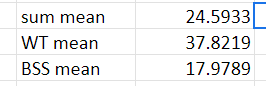
\includegraphics[width=2.77083in,height=0.89583in]{media/image25.png}

\subsection{Graphs}\label{graphs}

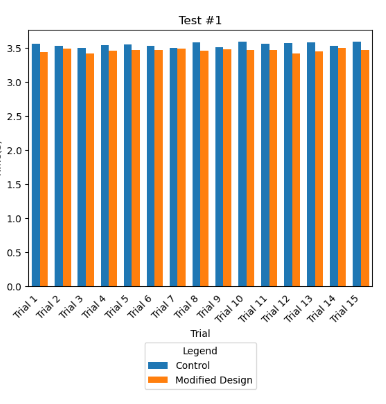
\includegraphics[width=5.40982in,height=5.66208in]{media/image2.png}

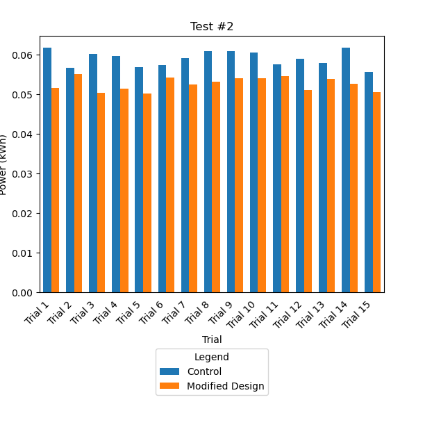
\includegraphics[width=5.40983in,height=5.57687in]{media/image11.png}

\subsection{Statistical Analysis}\label{statistical-analysis}

Type of statistical analysis (t-test, chi square test, ANOVA, etc):
Z-test

Degrees of freedom: 2

Critical Value: 1.645

P Values: 0.034 and \textless0.001

Summary statement: The null hypothesis was rejected because the p-value
obtained was lesser than the 0.05 cutoff for the experiment. The null
hypothesis fails to hold.

\subsection[Photo Documentation]{\texorpdfstring{Photo
Documentation\protect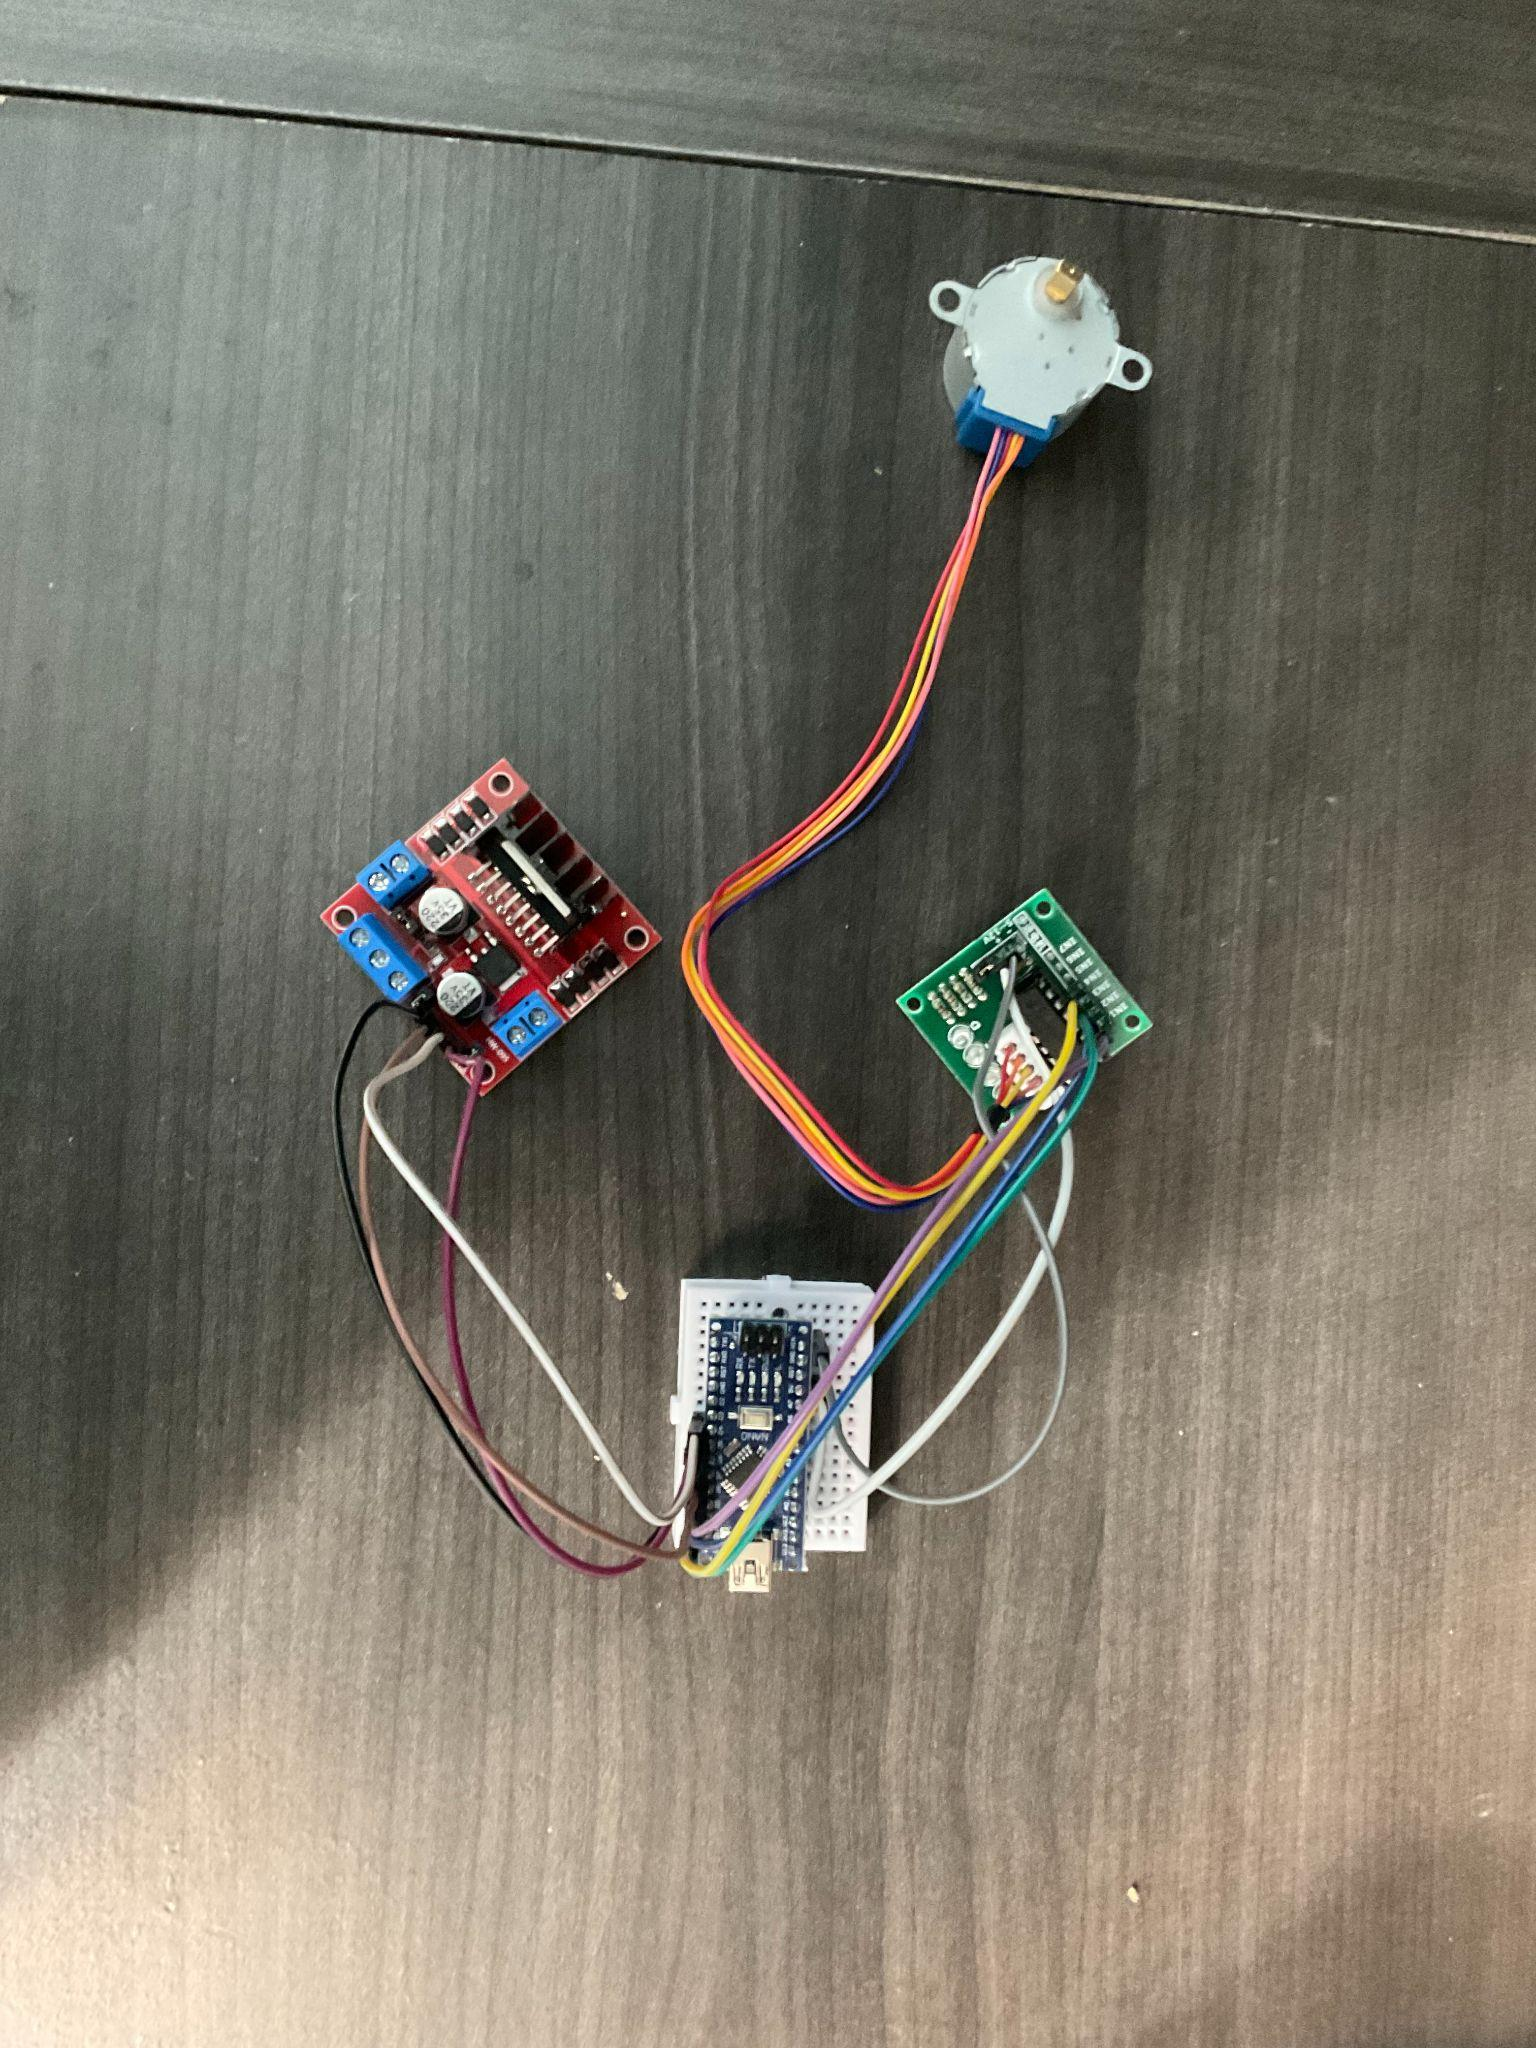
\includegraphics[width=3.08333in,height=4.38322in]{media/image46.jpg}\protect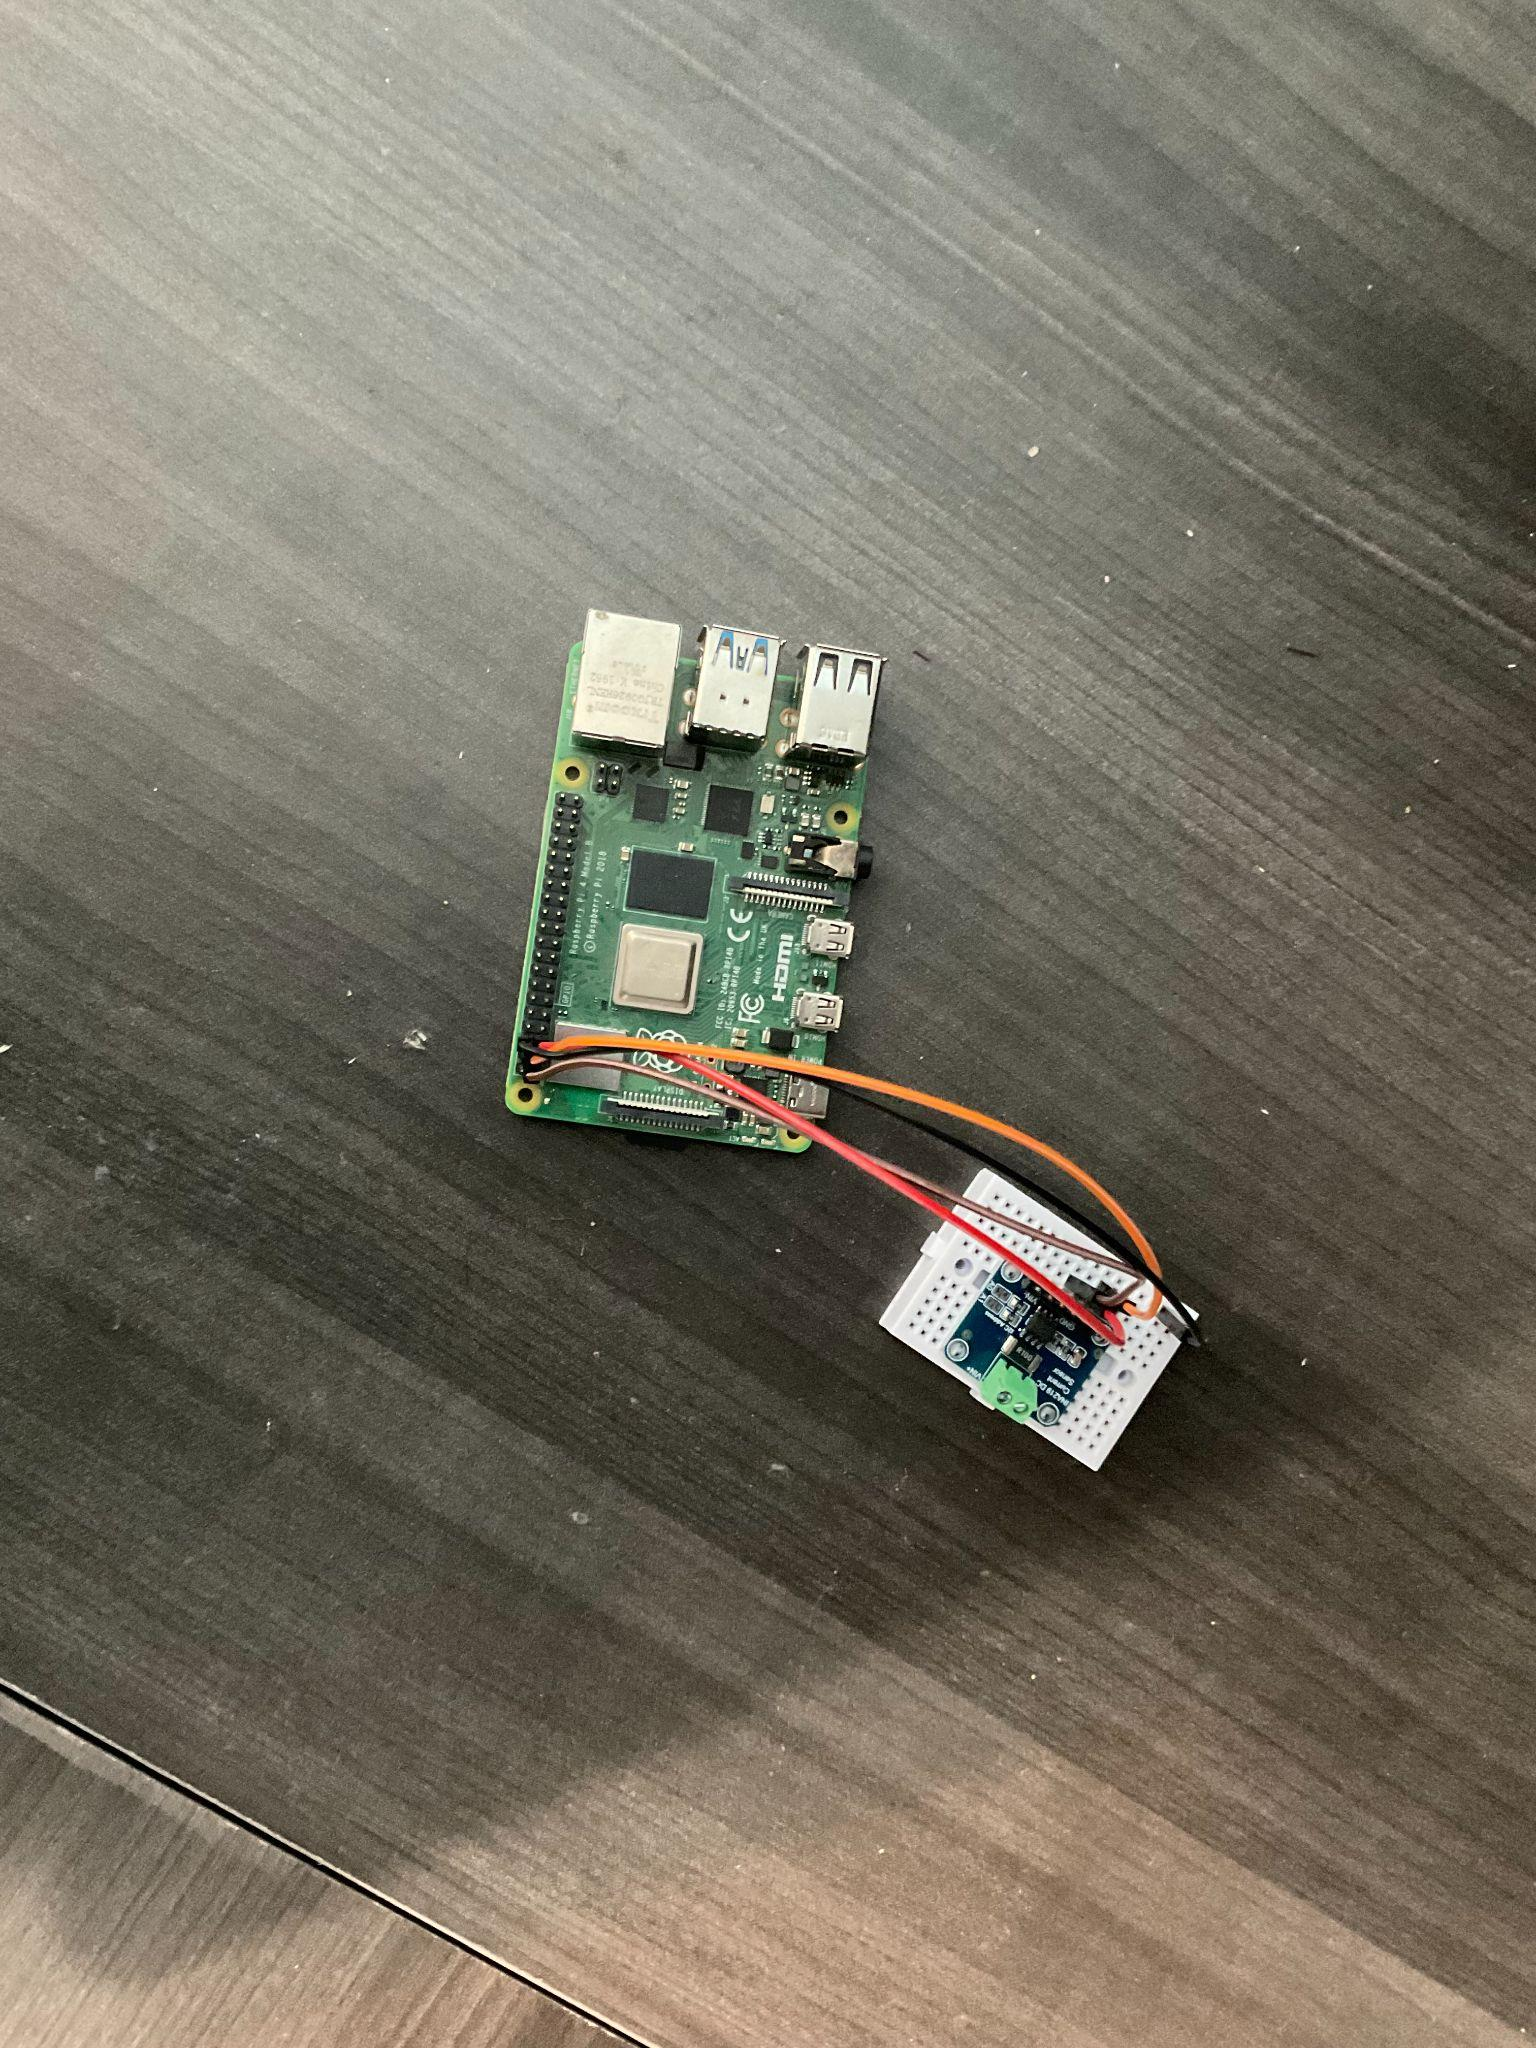
\includegraphics[width=4in,height=4.55967in]{media/image49.jpg}}{Photo Documentation}}\label{photo-documentation}

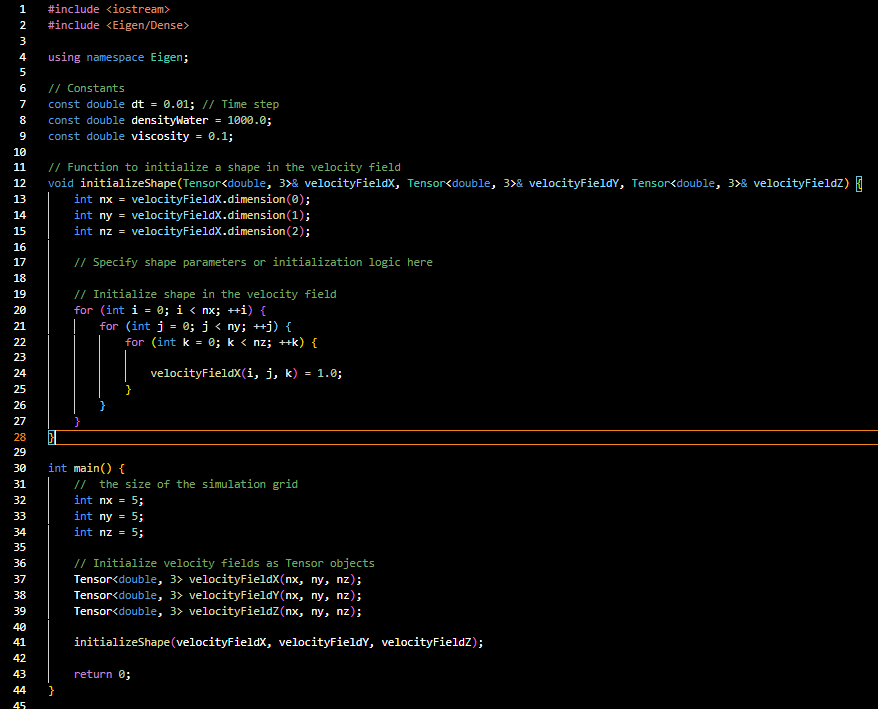
\includegraphics[width=5.021in,height=4.04492in]{media/image35.png}

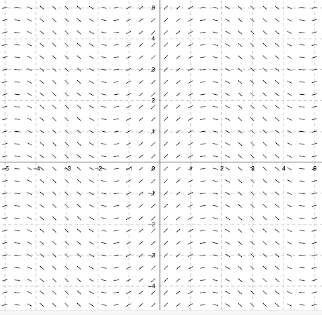
\includegraphics[width=2.09225in,height=2.0625in]{media/image16.png}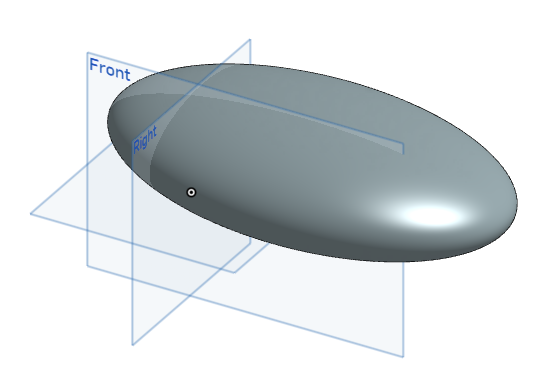
\includegraphics[width=2.61458in,height=1.85578in]{media/image30.png}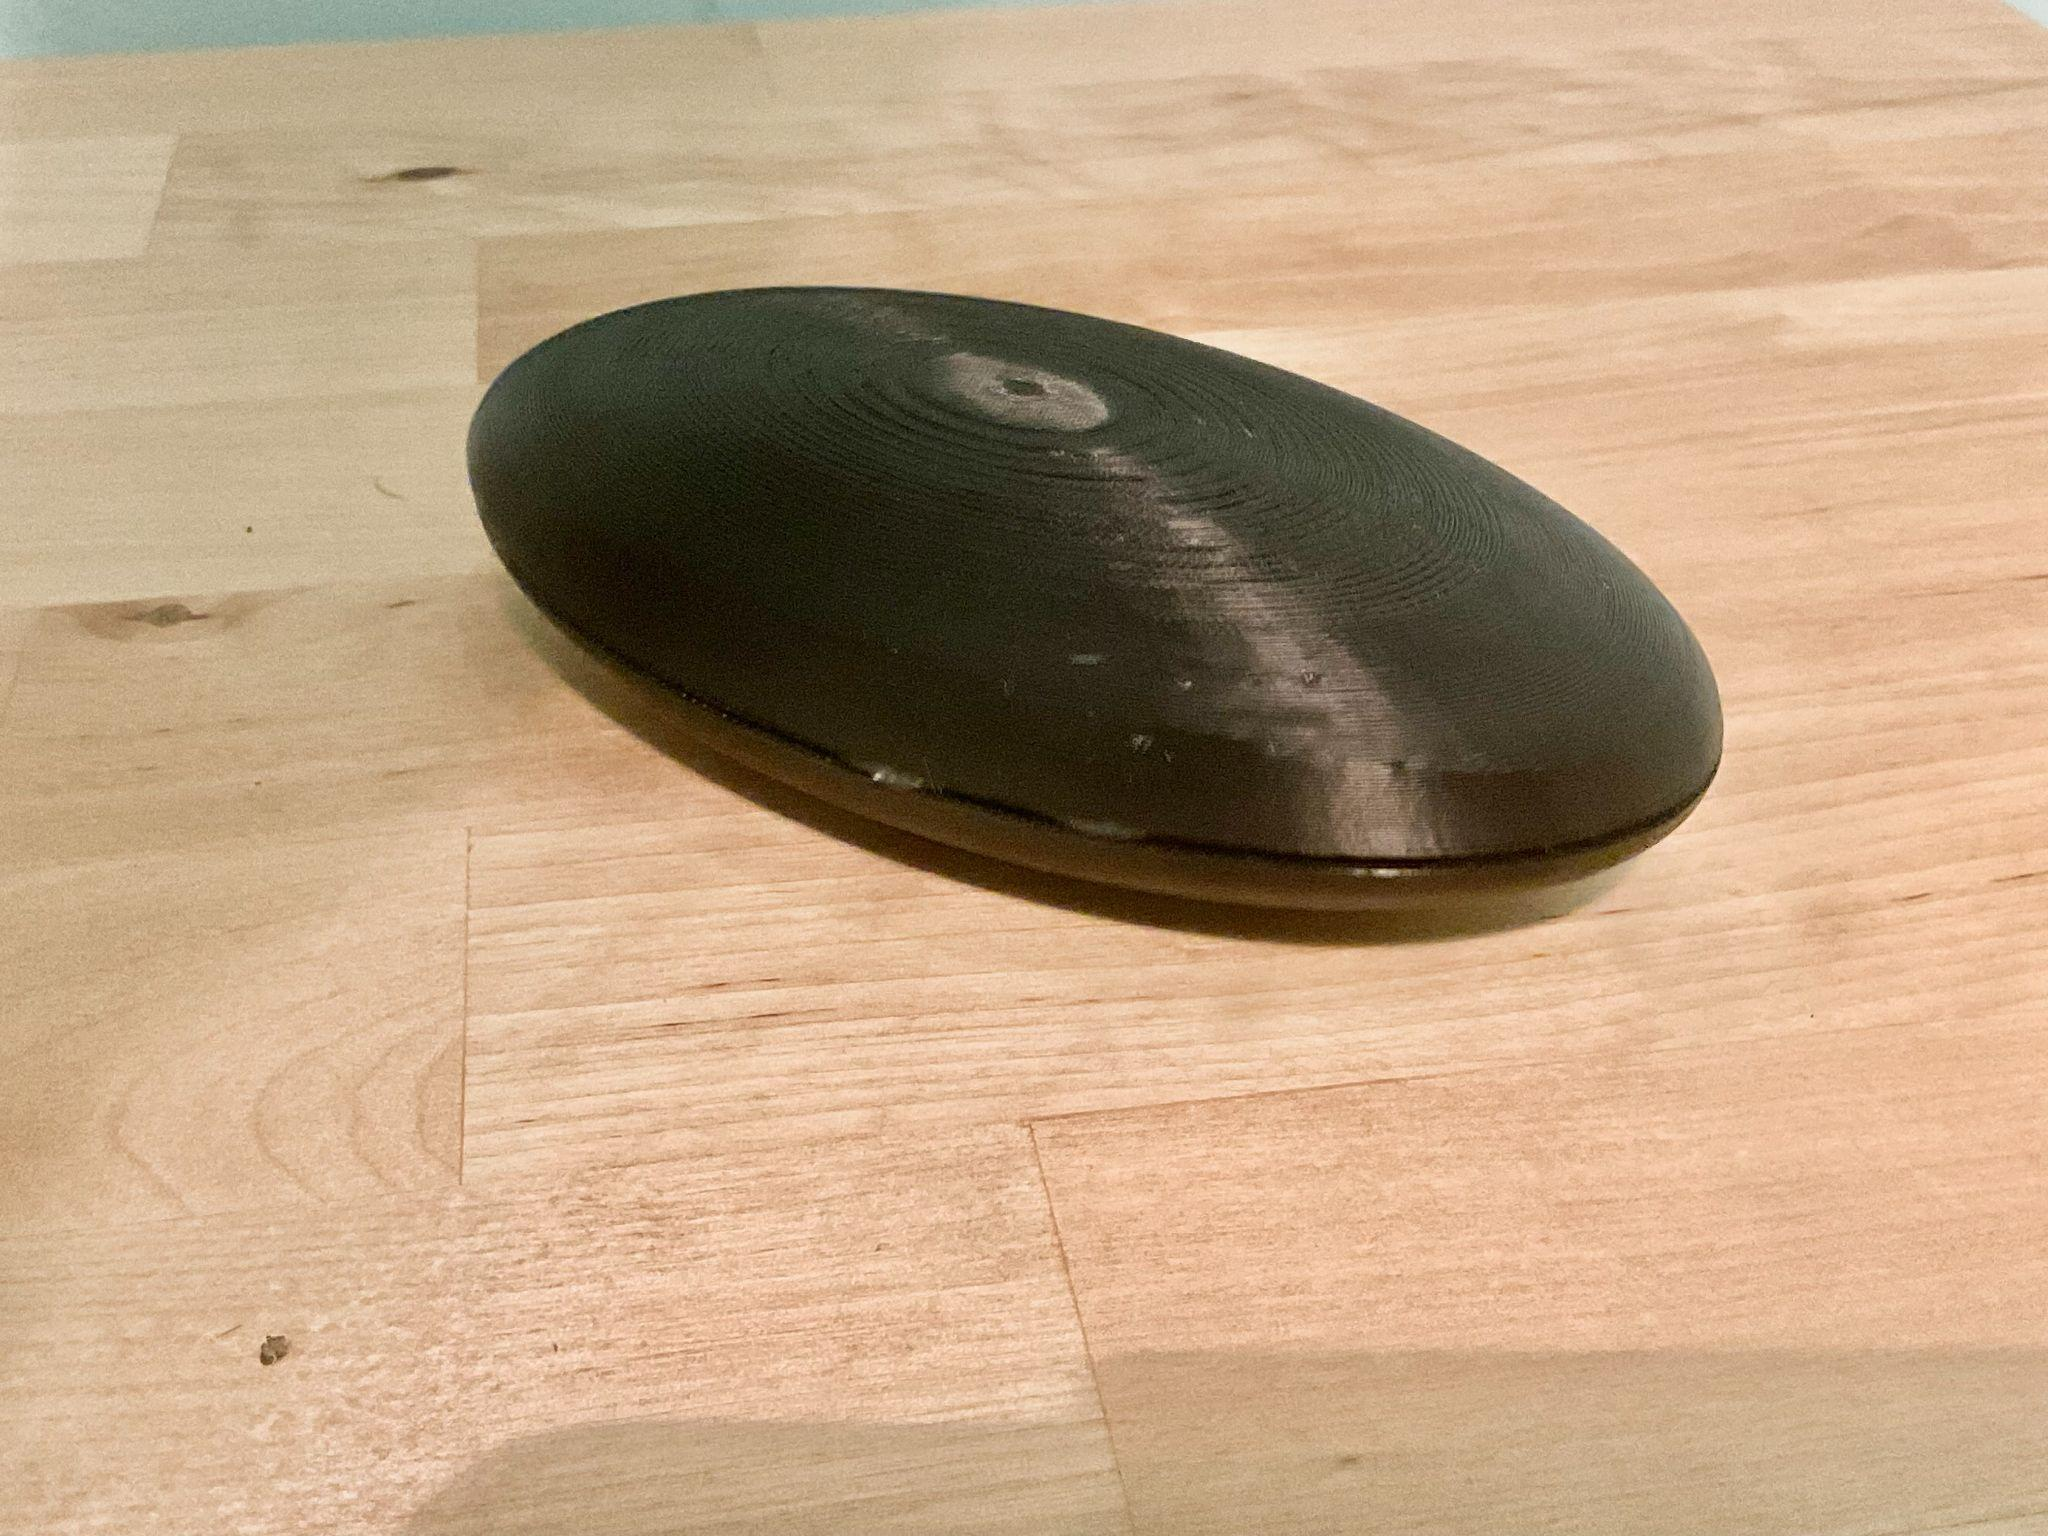
\includegraphics[width=3.22762in,height=1.66357in]{media/image47.jpg}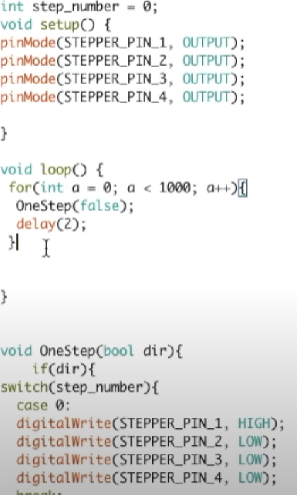
\includegraphics[width=2.49063in,height=4.15104in]{media/image20.png}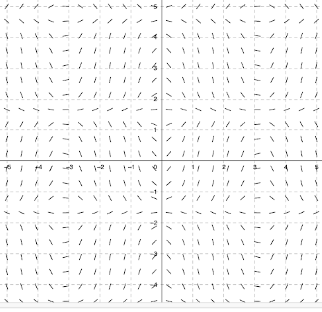
\includegraphics[width=2.23385in,height=2.16667in]{media/image13.png}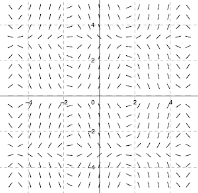
\includegraphics[width=2.17323in,height=2.10397in]{media/image3.png}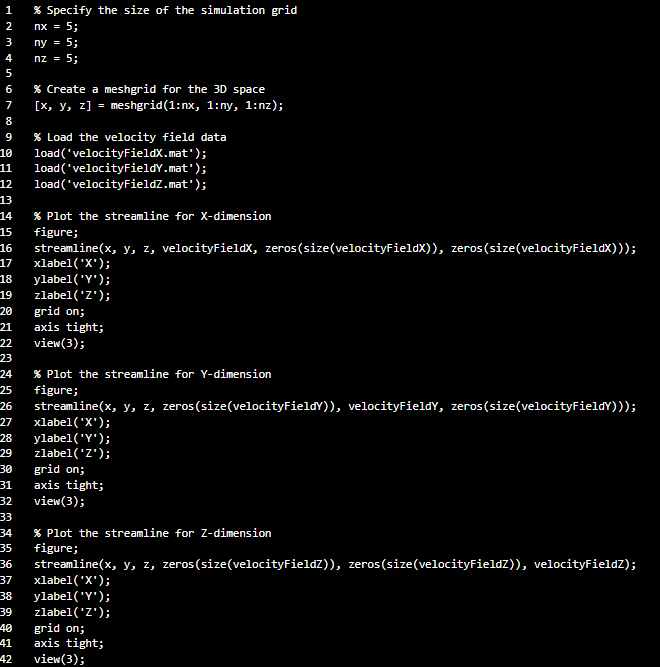
\includegraphics[width=3.99542in,height=4.04167in]{media/image27.png}

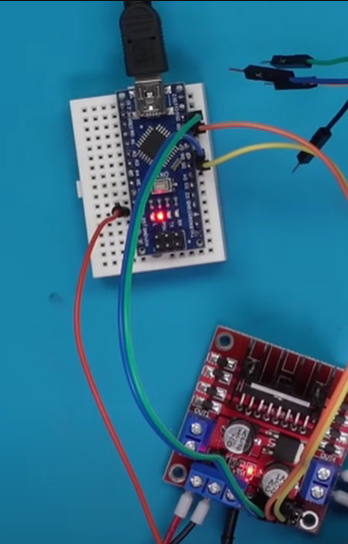
\includegraphics[width=3.625in,height=5.66667in]{media/image34.png}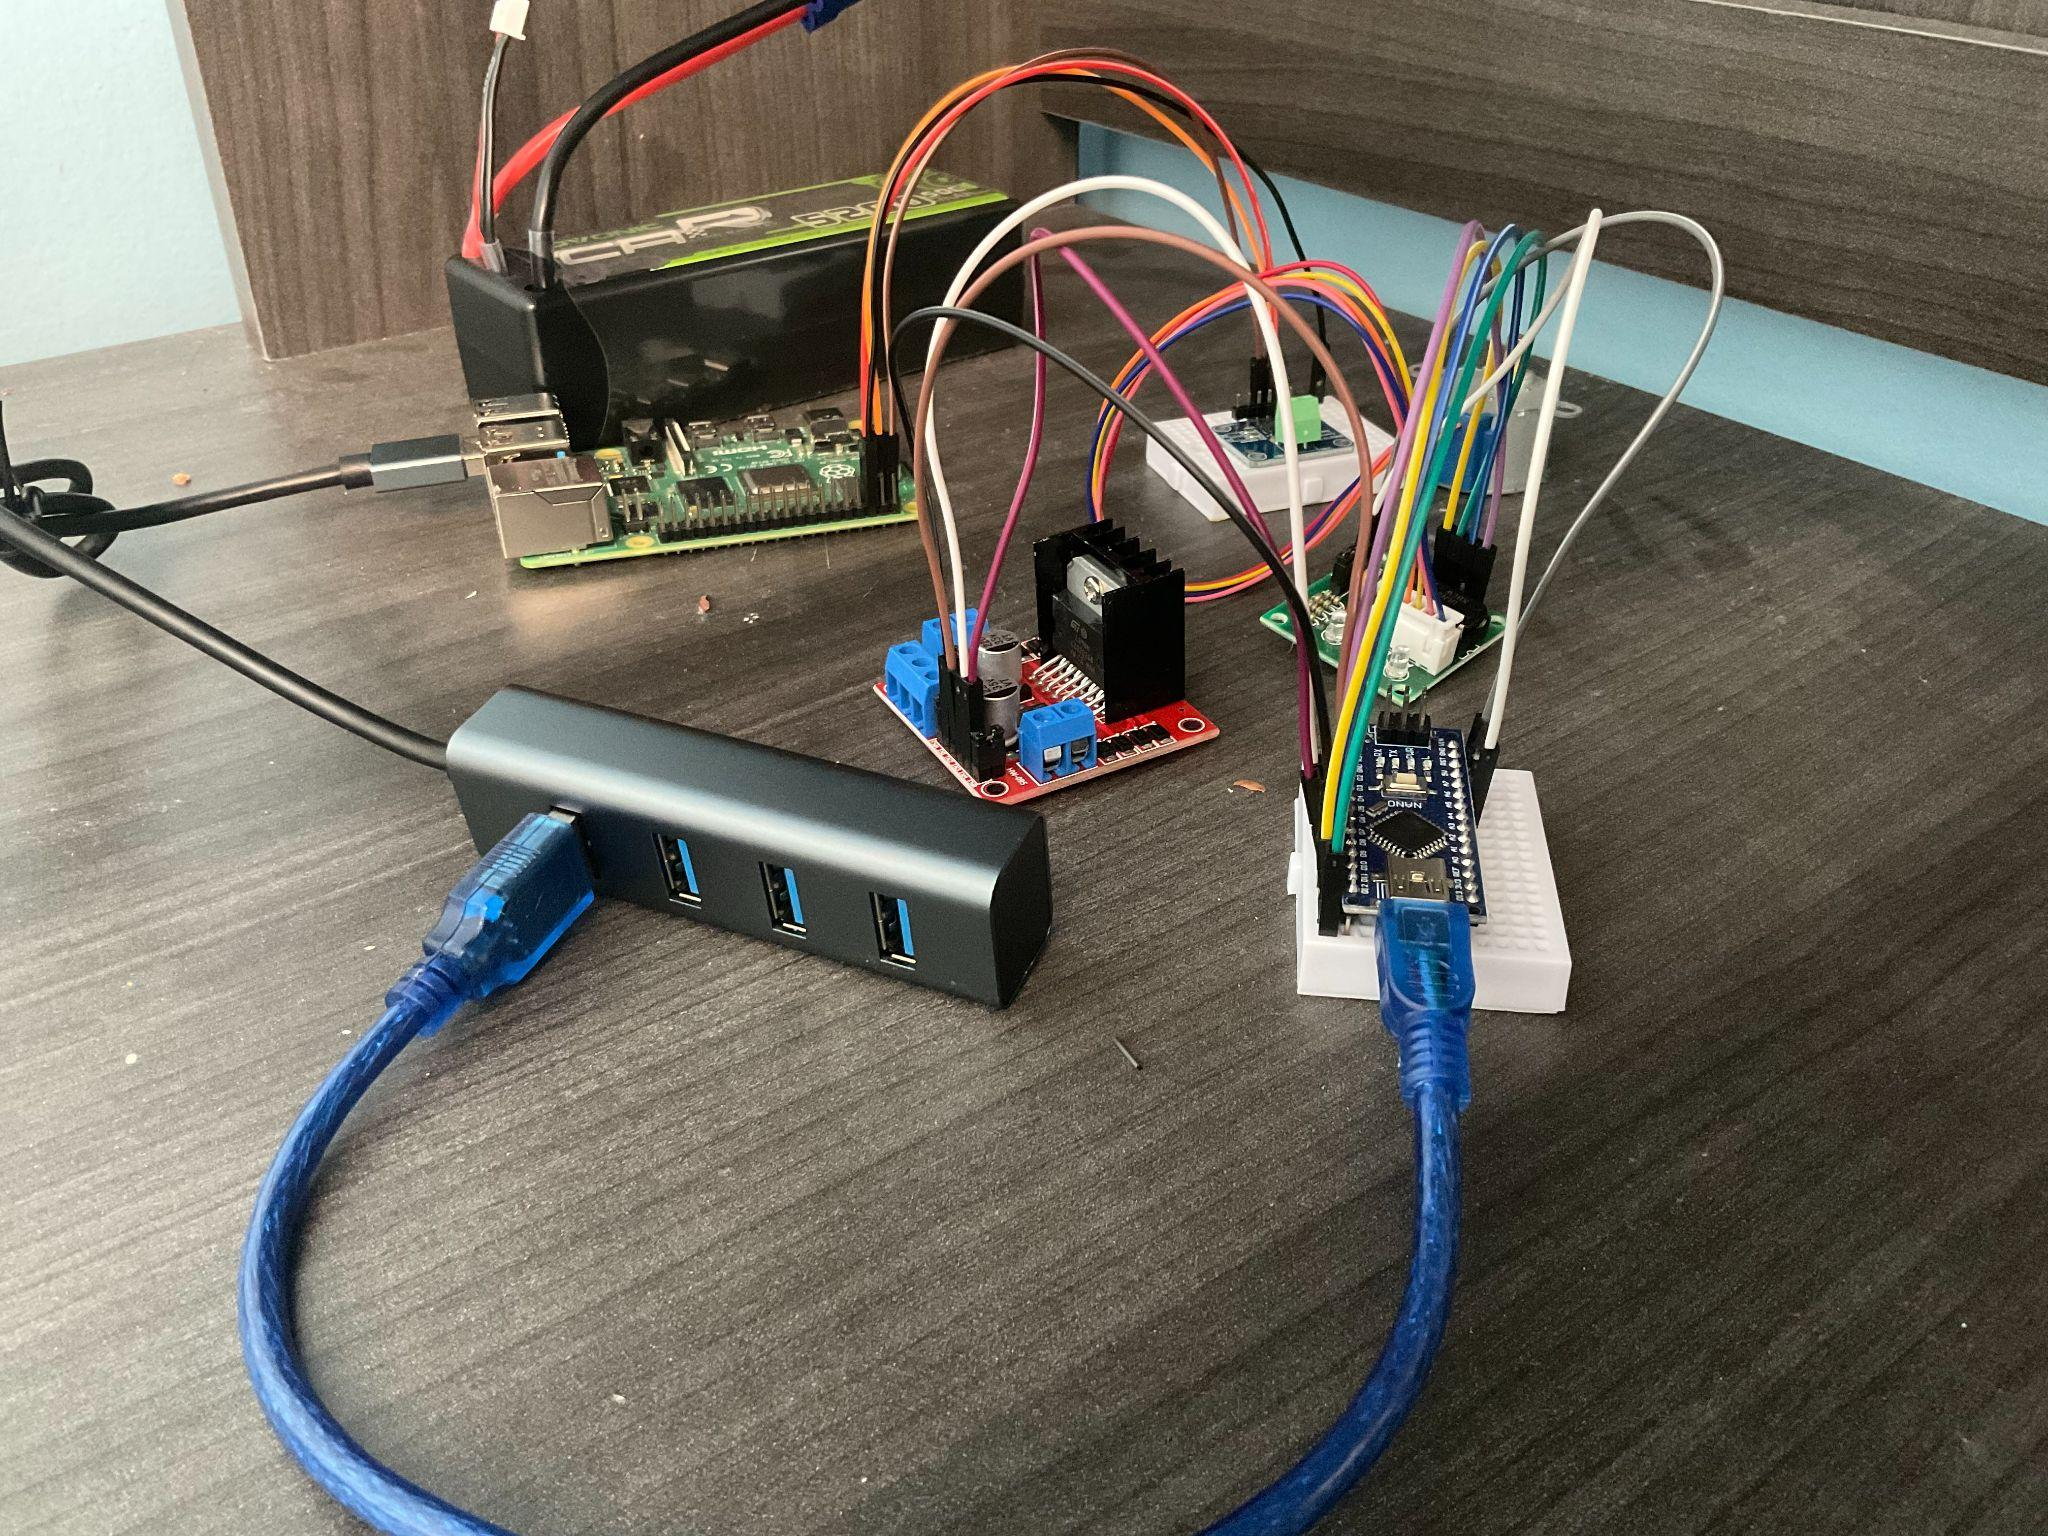
\includegraphics[width=4.73785in,height=3.41724in]{media/image48.jpg}

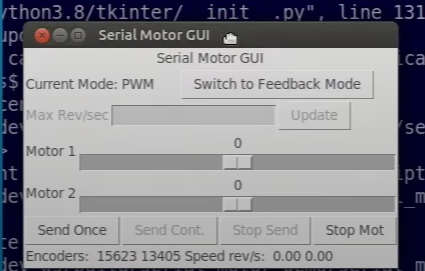
\includegraphics[width=4.22917in,height=3.05751in]{media/image26.png}

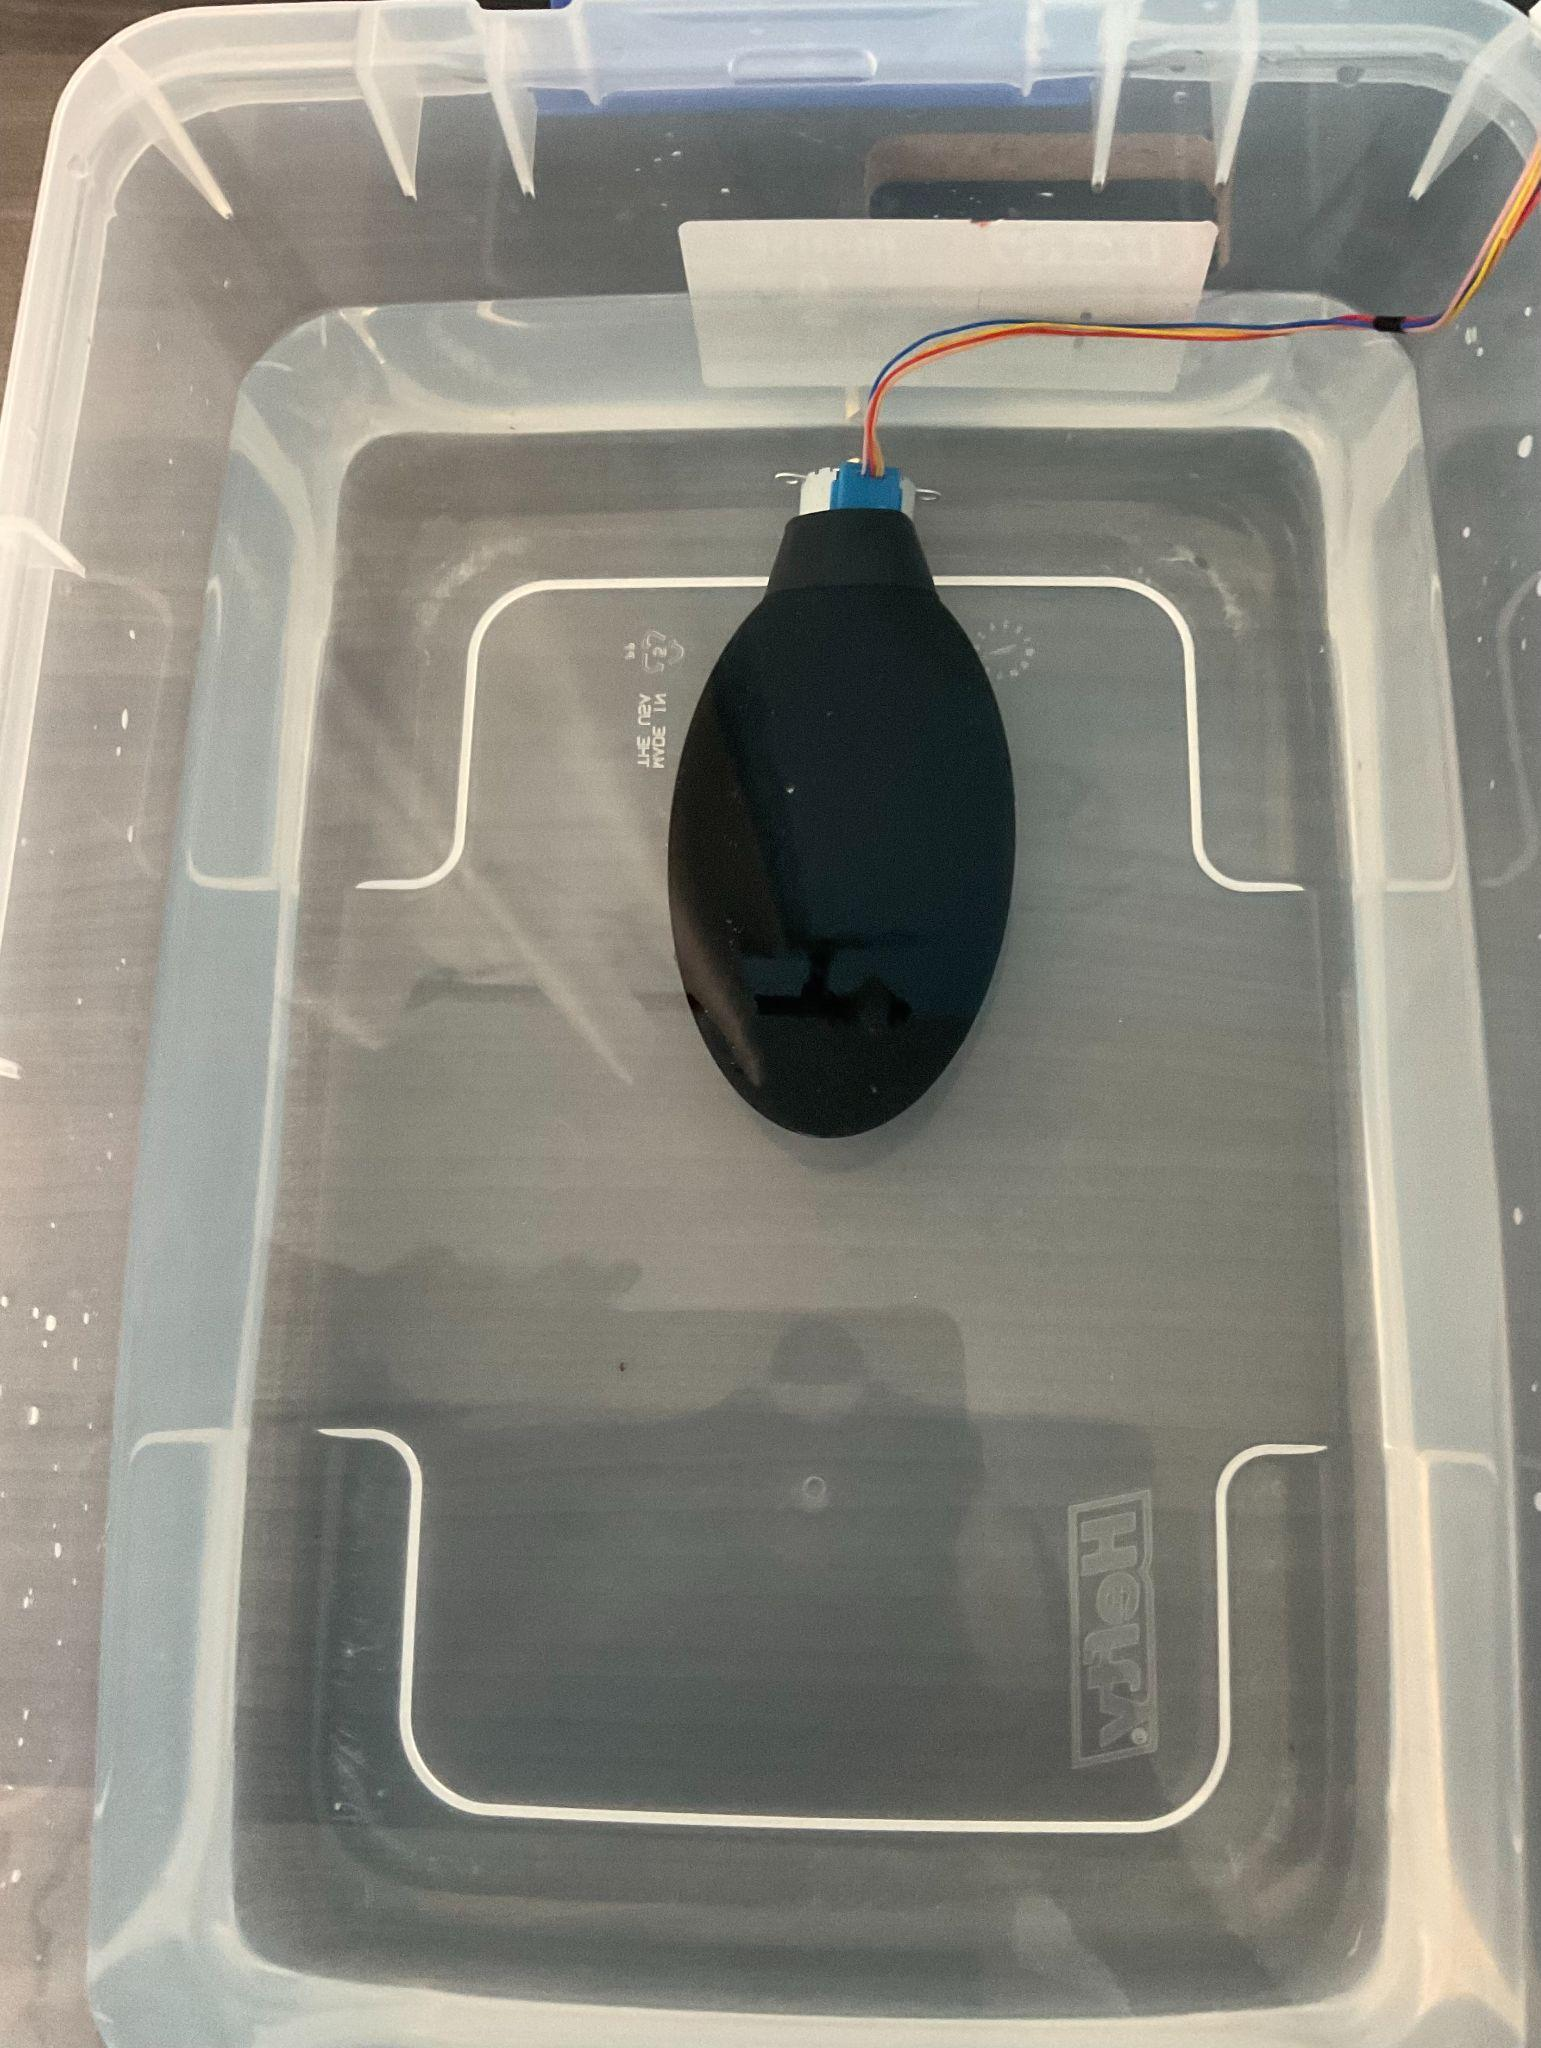
\includegraphics[width=4.86874in,height=4.03302in]{media/image45.jpg}

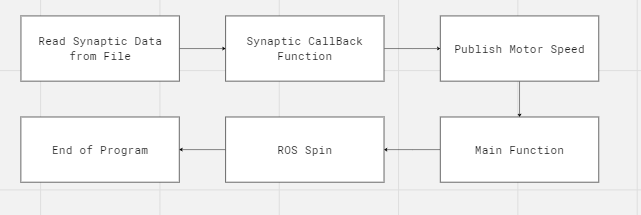
\includegraphics[width=6.67708in,height=2.23958in]{media/image7.png}

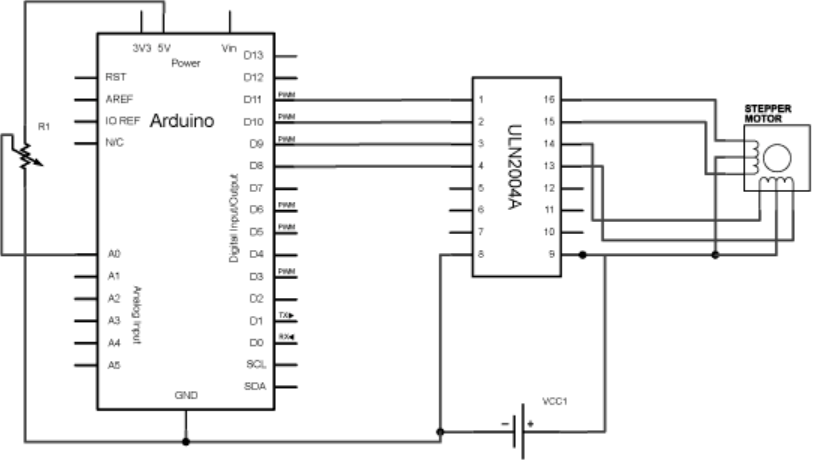
\includegraphics[width=7.84028in,height=4.40278in]{media/image24.png}

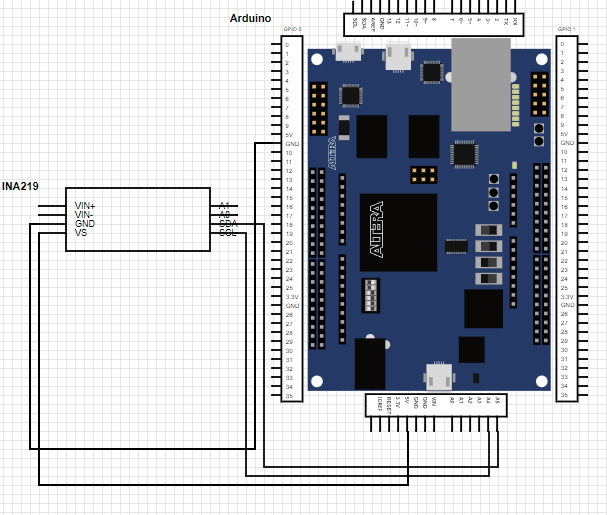
\includegraphics[width=6.32292in,height=5.36458in]{media/image29.png}

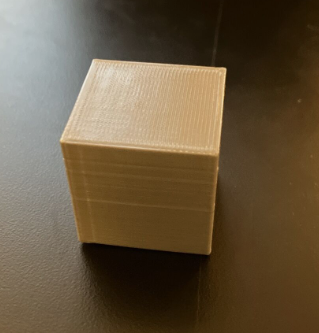
\includegraphics[width=3.32292in,height=3.46875in]{media/image36.png}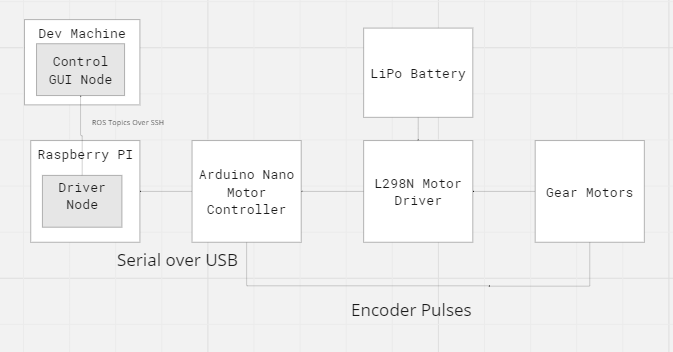
\includegraphics[width=7.01042in,height=3.66667in]{media/image38.png}